\cohead{\Large\textbf{Scheitelform}}
\fakesubsection{Scheitelform}
\begin{minipage}{\textwidth}
\settototalheight{\imgheight}{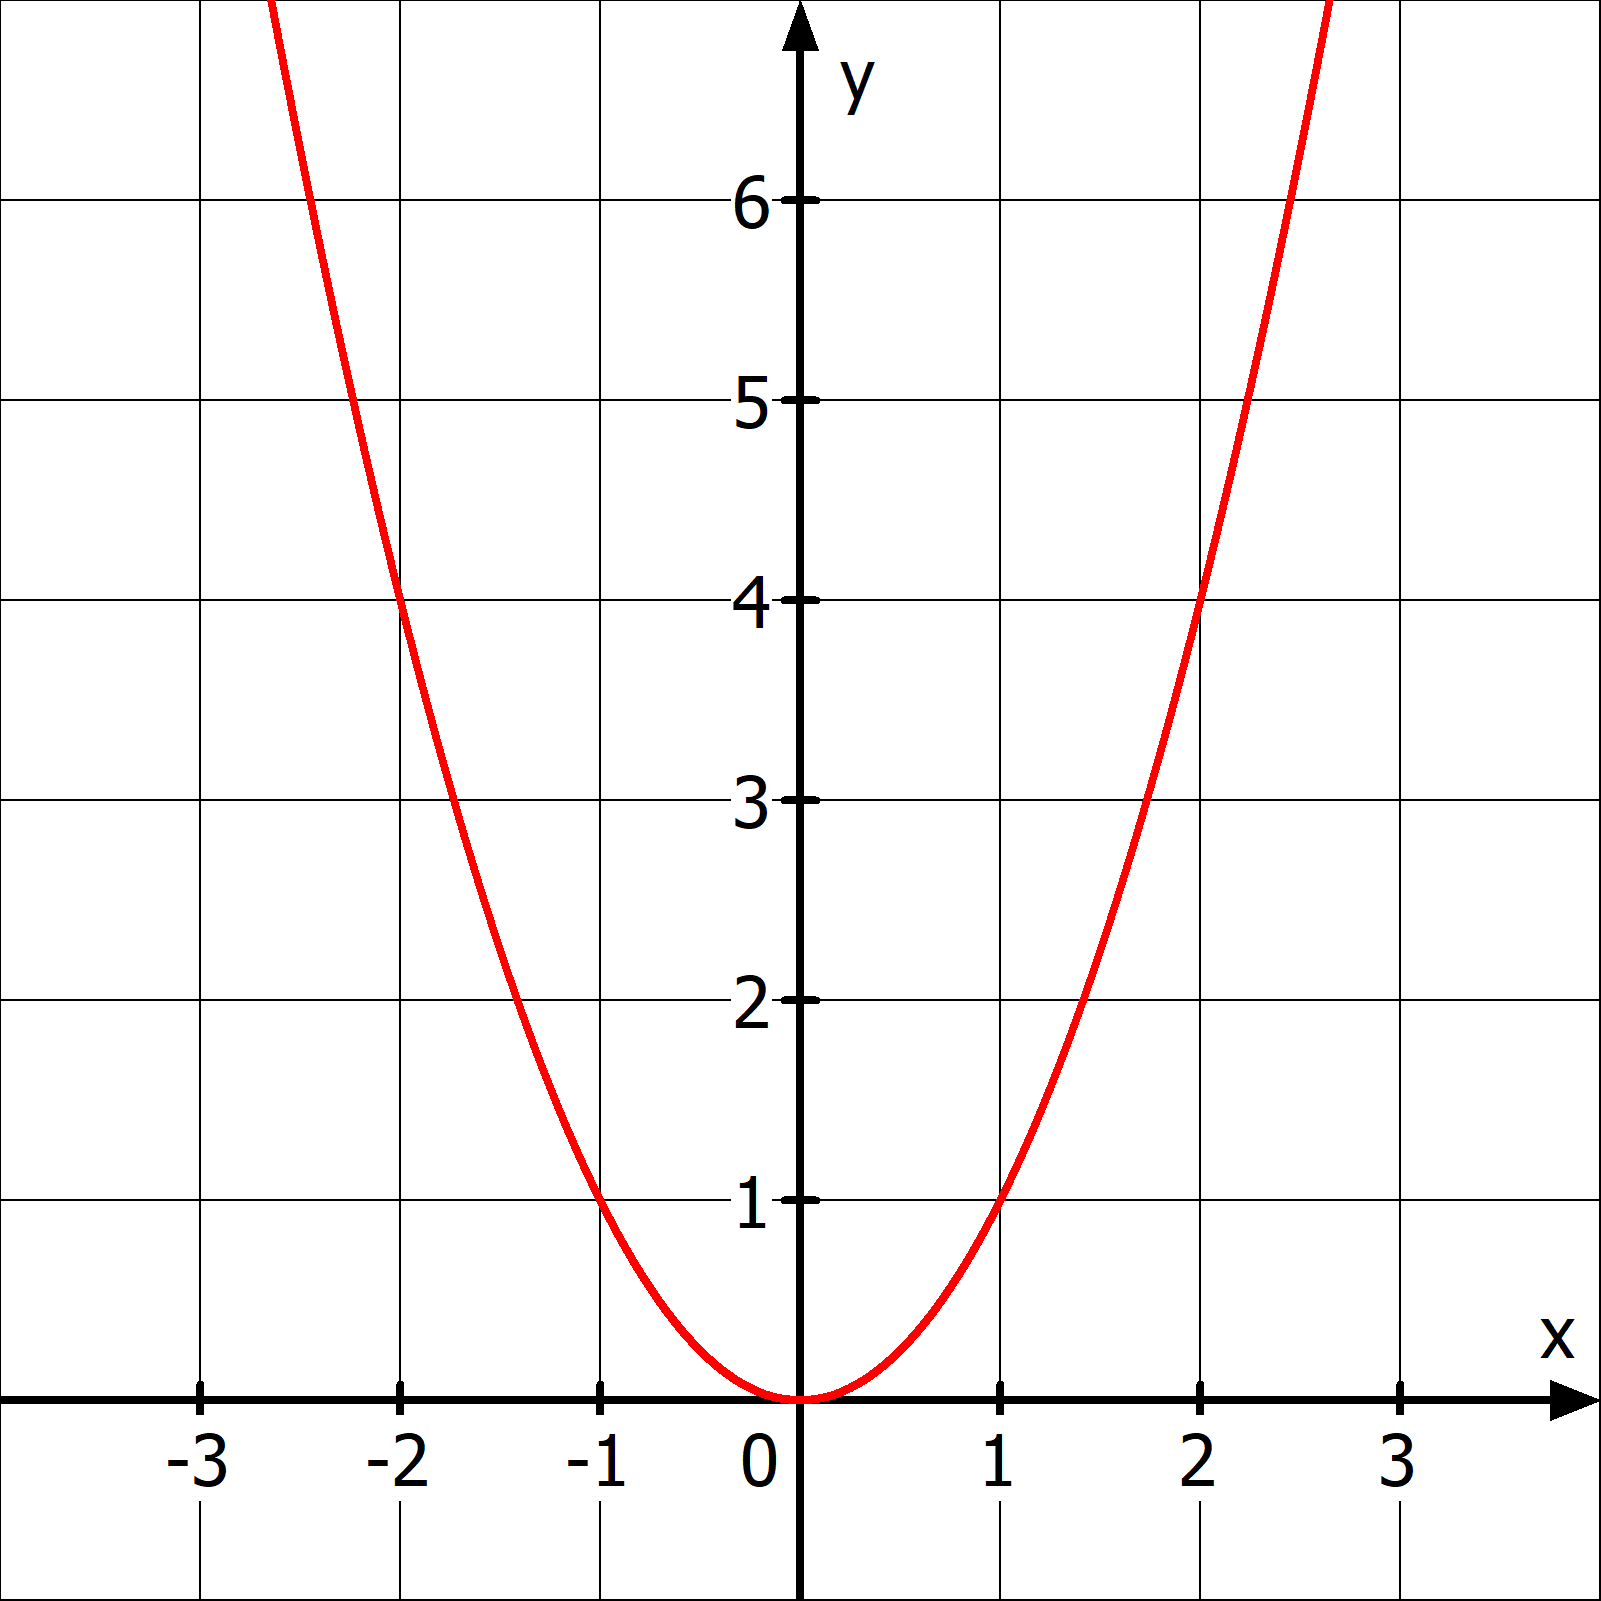
\includegraphics[width=0.5\textwidth]{\quadFkt/pics/normalparabel.png}}%
\adjustbox{valign=t}{\begin{minipage}{0.5\textwidth}%
        \iftoggle{qrcode}{%
            \setlength{\qrheight}{2.5cm}%
            \href{https://www.geogebra.org/m/tzeupua3}{
\includegraphics[width=\qrheight]{\quadFkt/pics/ScheitelformQR.png}}%
        }{%
            \vspace{2.5cm+\baselineskip}%
        }%

        {\centering\Large\textcolor{loes}{Das Schaubild der Funktion}%

        \textcolor{loes}{\(f(x)=x^2\)}%

        \textcolor{loes}{bezeichnet man als Normalparabel.}}%
\end{minipage}}%
\adjustbox{valign=t}{\begin{minipage}{0.5\textwidth}
	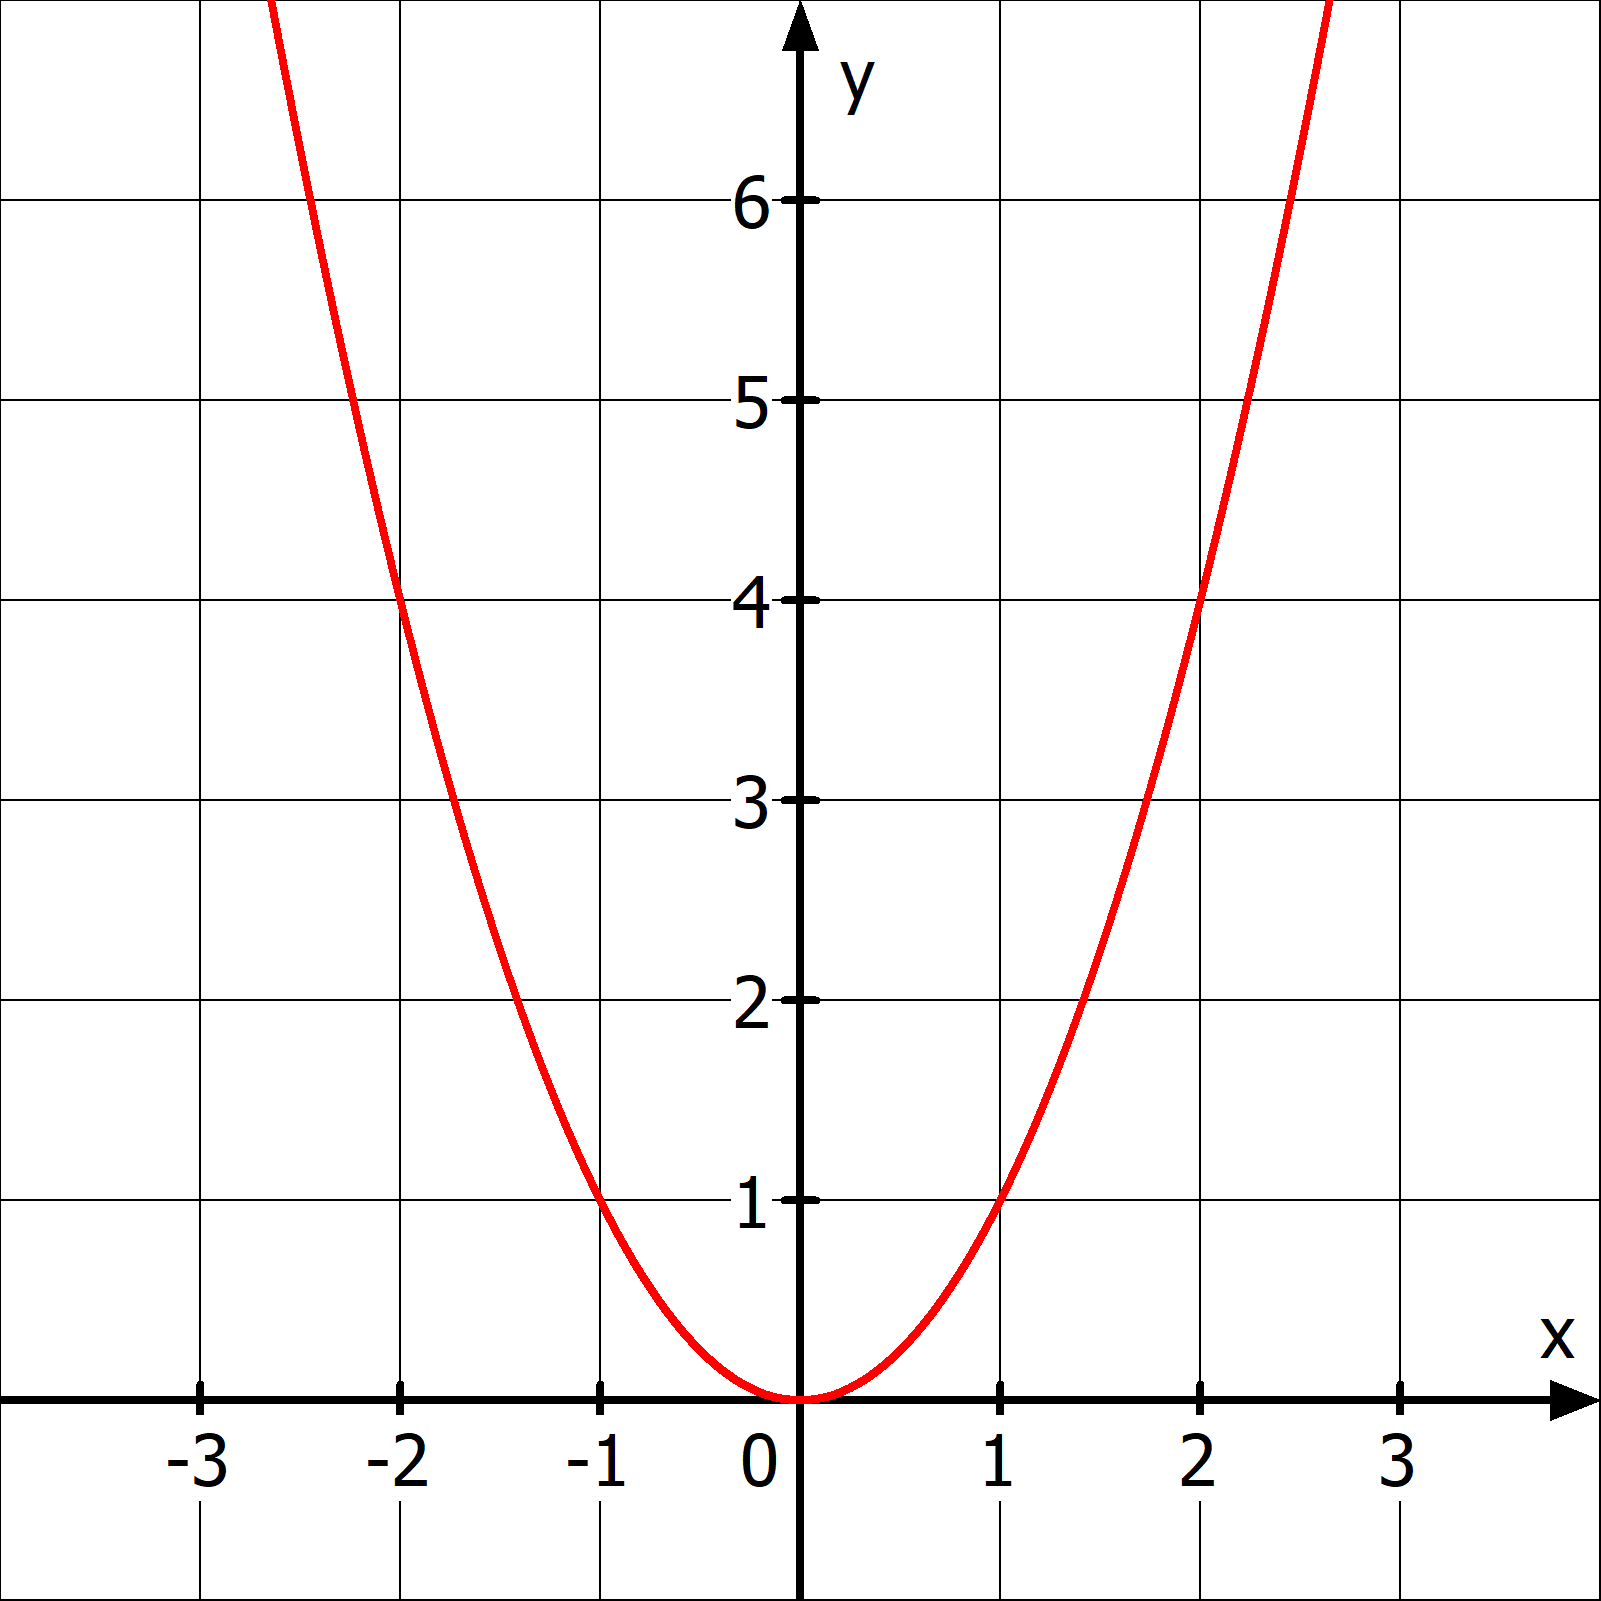
\includegraphics[width=\textwidth]{\quadFkt/pics/normalparabel.png}
\end{minipage}}%
\end{minipage}
\textbf{Verschieben in y-Richtung}
\begin{tcolorbox}\centering
	\(\textcolor{loestc}{f(x)=x^2+y_S}\)
\end{tcolorbox}
\textcolor{loes}{Für \(y_S>0\) wird die Parabel nach oben verschoben, für \(y_S<0\) wird die Parabel nach unten verschoben.}

\bigskip

\textbf{Verschieben in x-Richtung}
\begin{tcolorbox}\centering
	\(\textcolor{loestc}{f(x)=\left(x-x_S\right)^2}\)
\end{tcolorbox}
\textcolor{loes}{Für \(x_S>0\) wird die Parabel nach rechts verschoben, für \(x_S<0\) wird die Parabel nach links verschoben.}

\bigskip

\textbf{Strecken und Stauchen in y-Richtung}
\begin{tcolorbox}\centering
	\(\textcolor{loestc}{f(x)=a\cdot x^2}\)
\end{tcolorbox}
\textcolor{loes}{Für \(a>1\) wird die Parabel gestreckt, sie erscheint dann schmäler.}

\textcolor{loes}{Für \(0<a<1\) wird die Parabel gestaucht, sie erscheint dann breiter.}

\textcolor{loes}{Für negative \(a\) wird die Parabel zusätzlich nach unten geklappt.}

\bigskip

\textbf{Scheitelform}
\begin{tcolorbox}\centering
	\(\textcolor{loestc}{f(x)=a\cdot \left(x-x_S\right)^2+y_S}\)
\end{tcolorbox}
\textcolor{loes}{Man kann die Parabel gleichzeitig in x-Richtung und y-Richtung verschieben sowie strecken oder stauchen. Man erhält so die Scheitelform. Liegt die Funktionsgleichung einer Parabel in der Scheitelform vor, so kann man den Scheitel \(S\left(x_S\middle\vert y_S \right)\) direkt ablesen.}\newpage
%%%%%%%%%%%%%%%%%%%%%%%%%%%%%%%%%%%%%%%%%
\cohead{\Large\textbf{Verschieben in y-Richtung}}
\begin{minipage}{\textwidth}
\begin{tabular}{cc}
	\begin{minipage}{0.47\textwidth}\centering\Large
		\textcolor{loes}{Die Normalparabel wird um 2 Einheiten nach unten verschoben.}

		\bigskip

		\textcolor{loes}{\(f(x)=x^2-2\)}

		\bigskip

		\textcolor{loes}{Der Scheitel liegt bei \(S\left(0\middle\vert -2\right)\)}
	\end{minipage}%
	&
	\begin{minipage}{0.47\textwidth}
		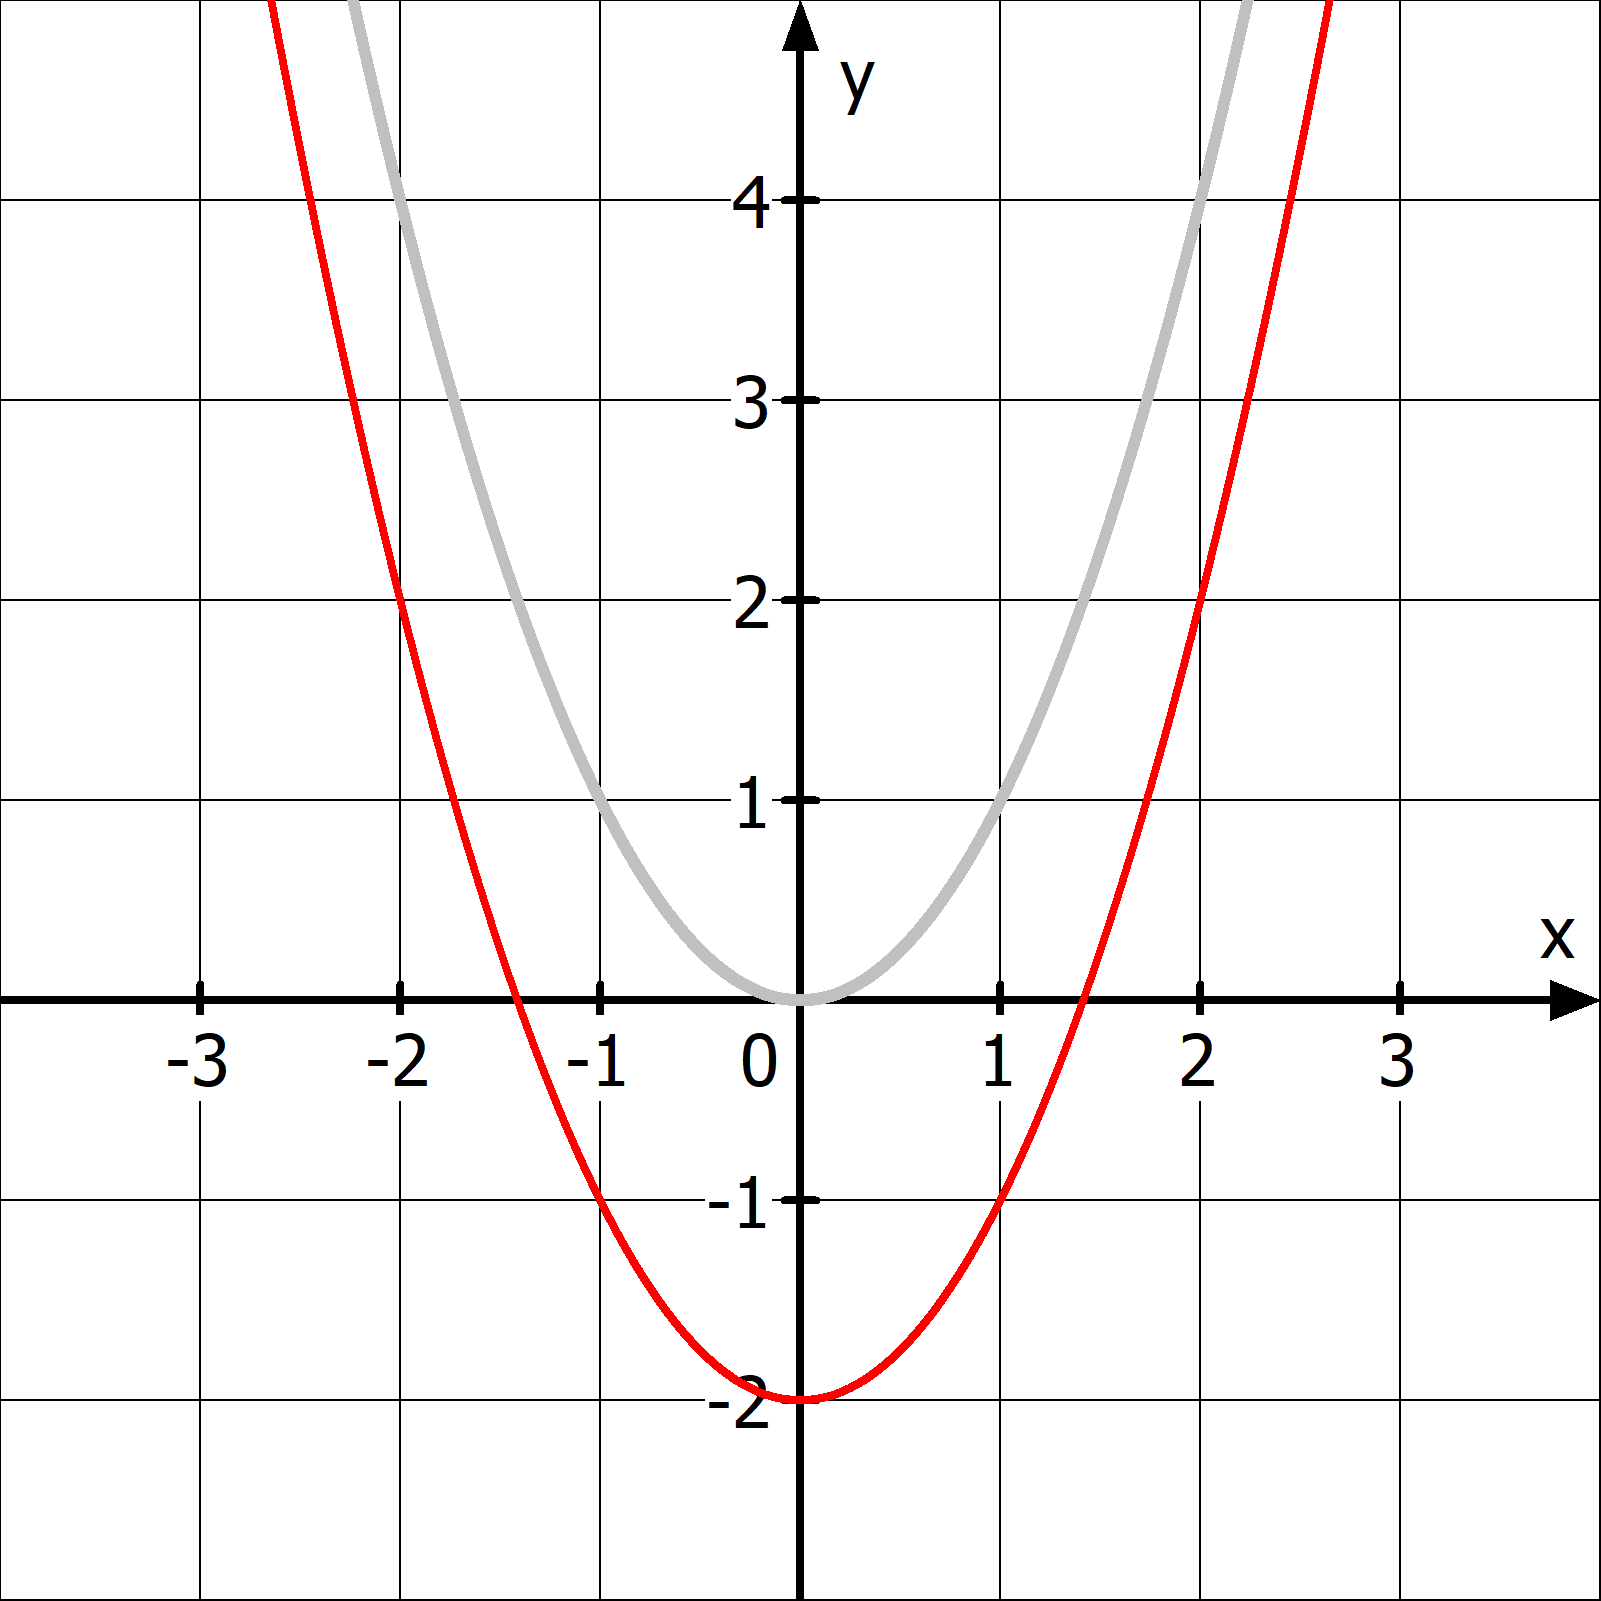
\includegraphics[width=\textwidth]{\quadFkt/pics/verschiebenY1.png}
	\end{minipage}%
	\\
	\midrule
	\begin{minipage}{0.47\textwidth}\centering\Large
		Die Normalparabel wird um 3 Einheiten nach oben verschoben.

		\bigskip

		\textcolor{loes}{\(f(x)=x^2+3\)}

		\bigskip

		\textcolor{loes}{Der Scheitel liegt bei \(S\left(0\middle\vert 3\right) \)}
	\end{minipage}%
	&
	\begin{minipage}{0.47\textwidth}
		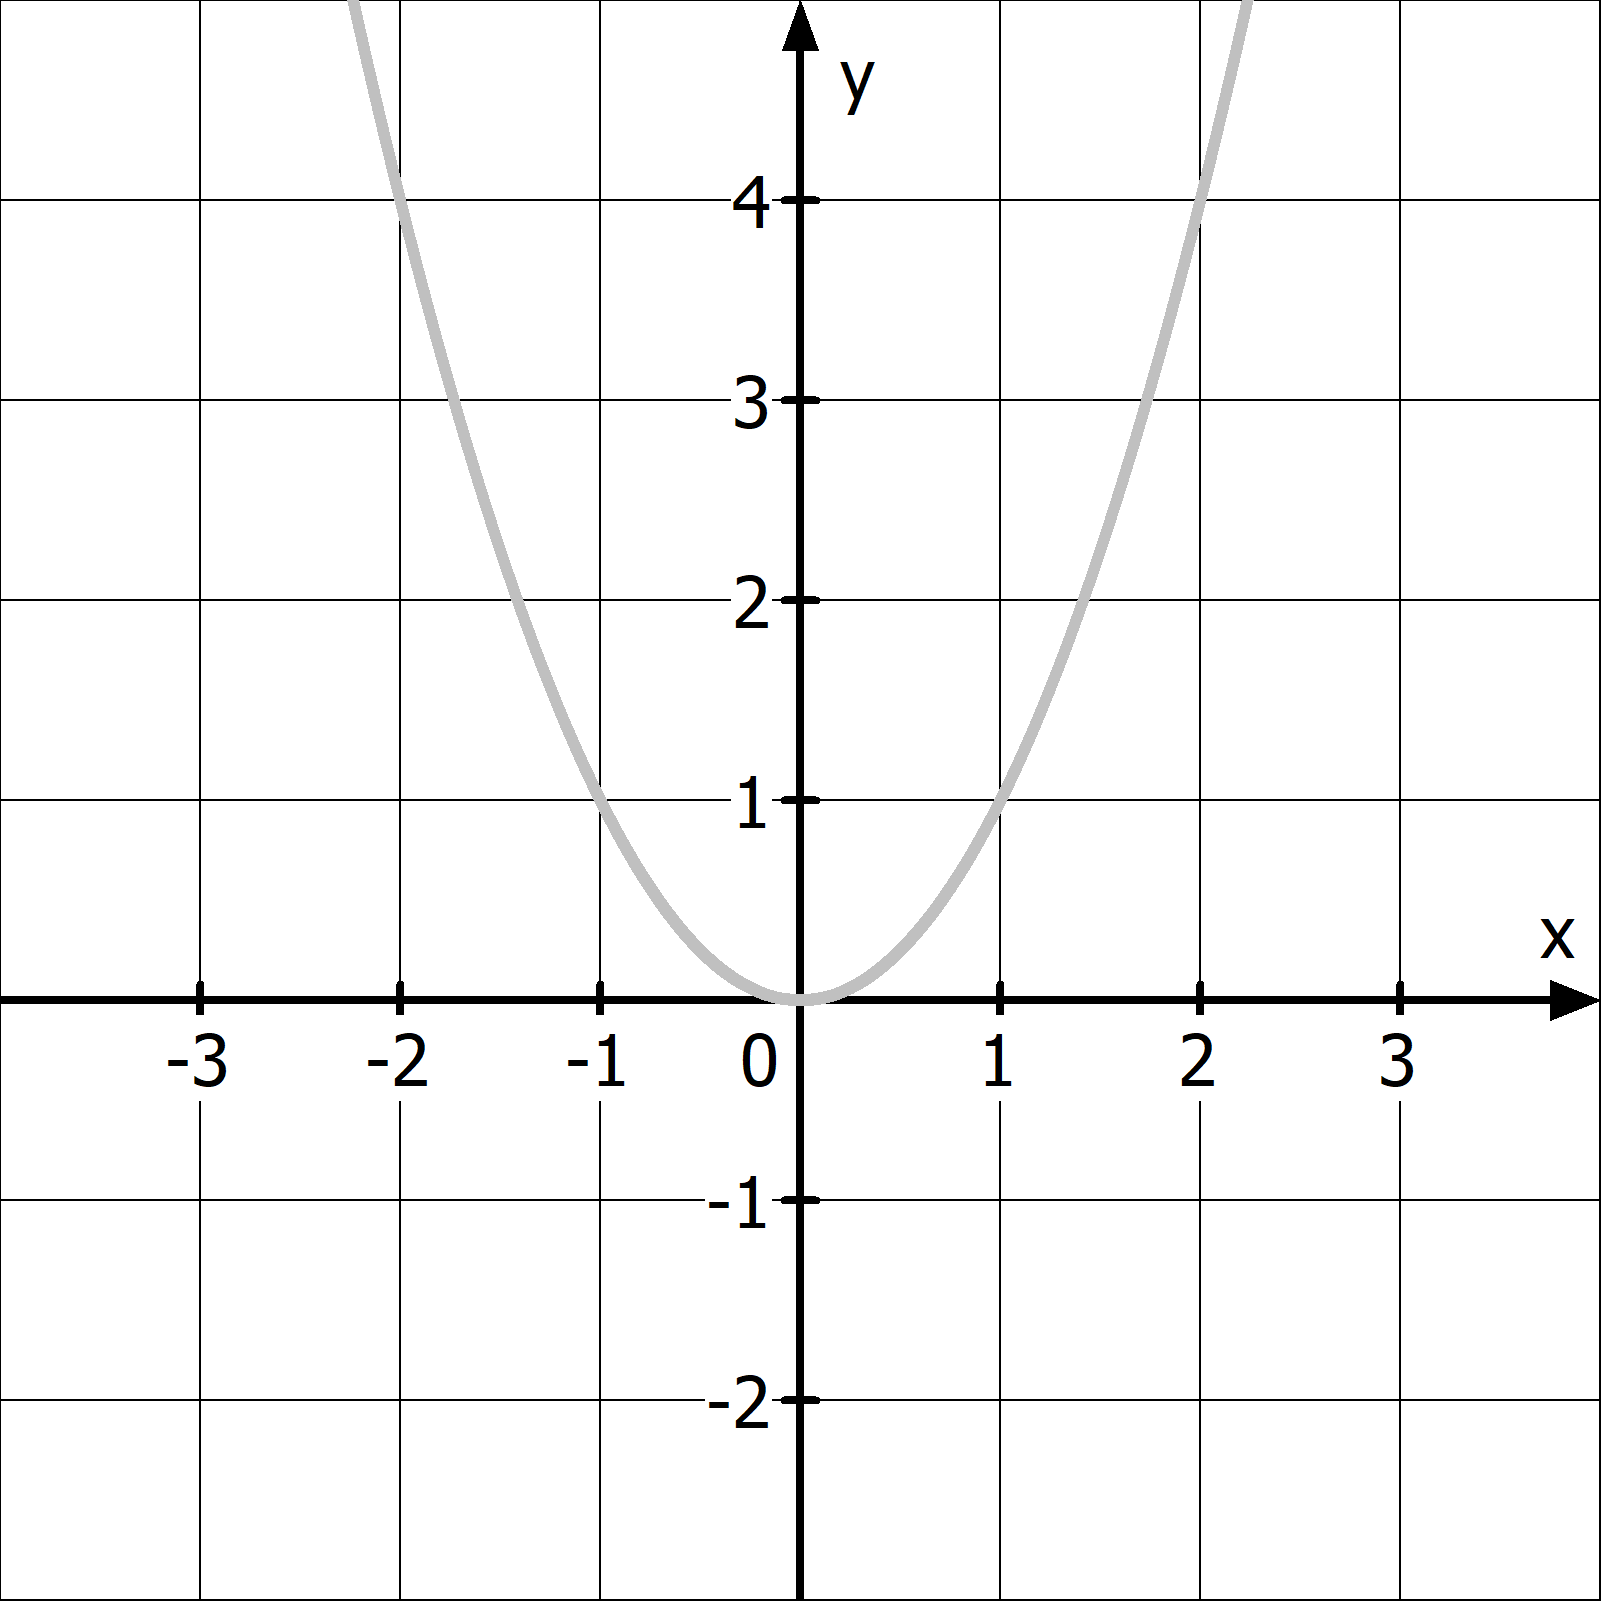
\includegraphics[width=\textwidth]{\quadFkt/pics/verschieben_empty.png}
	\end{minipage}%
	\\
	\midrule
	\begin{minipage}{0.47\textwidth}\centering\Large
		\textcolor{loes}{Die Normalparabel wird um 1 Einheit nach unten verschoben.}

		\bigskip

		\(f(x)=x^2-1\)

		\bigskip

		Der Scheitel liegt bei \(S\left(0\middle\vert -1\right)\)
	\end{minipage}%
	&
	\begin{minipage}{0.47\textwidth}
		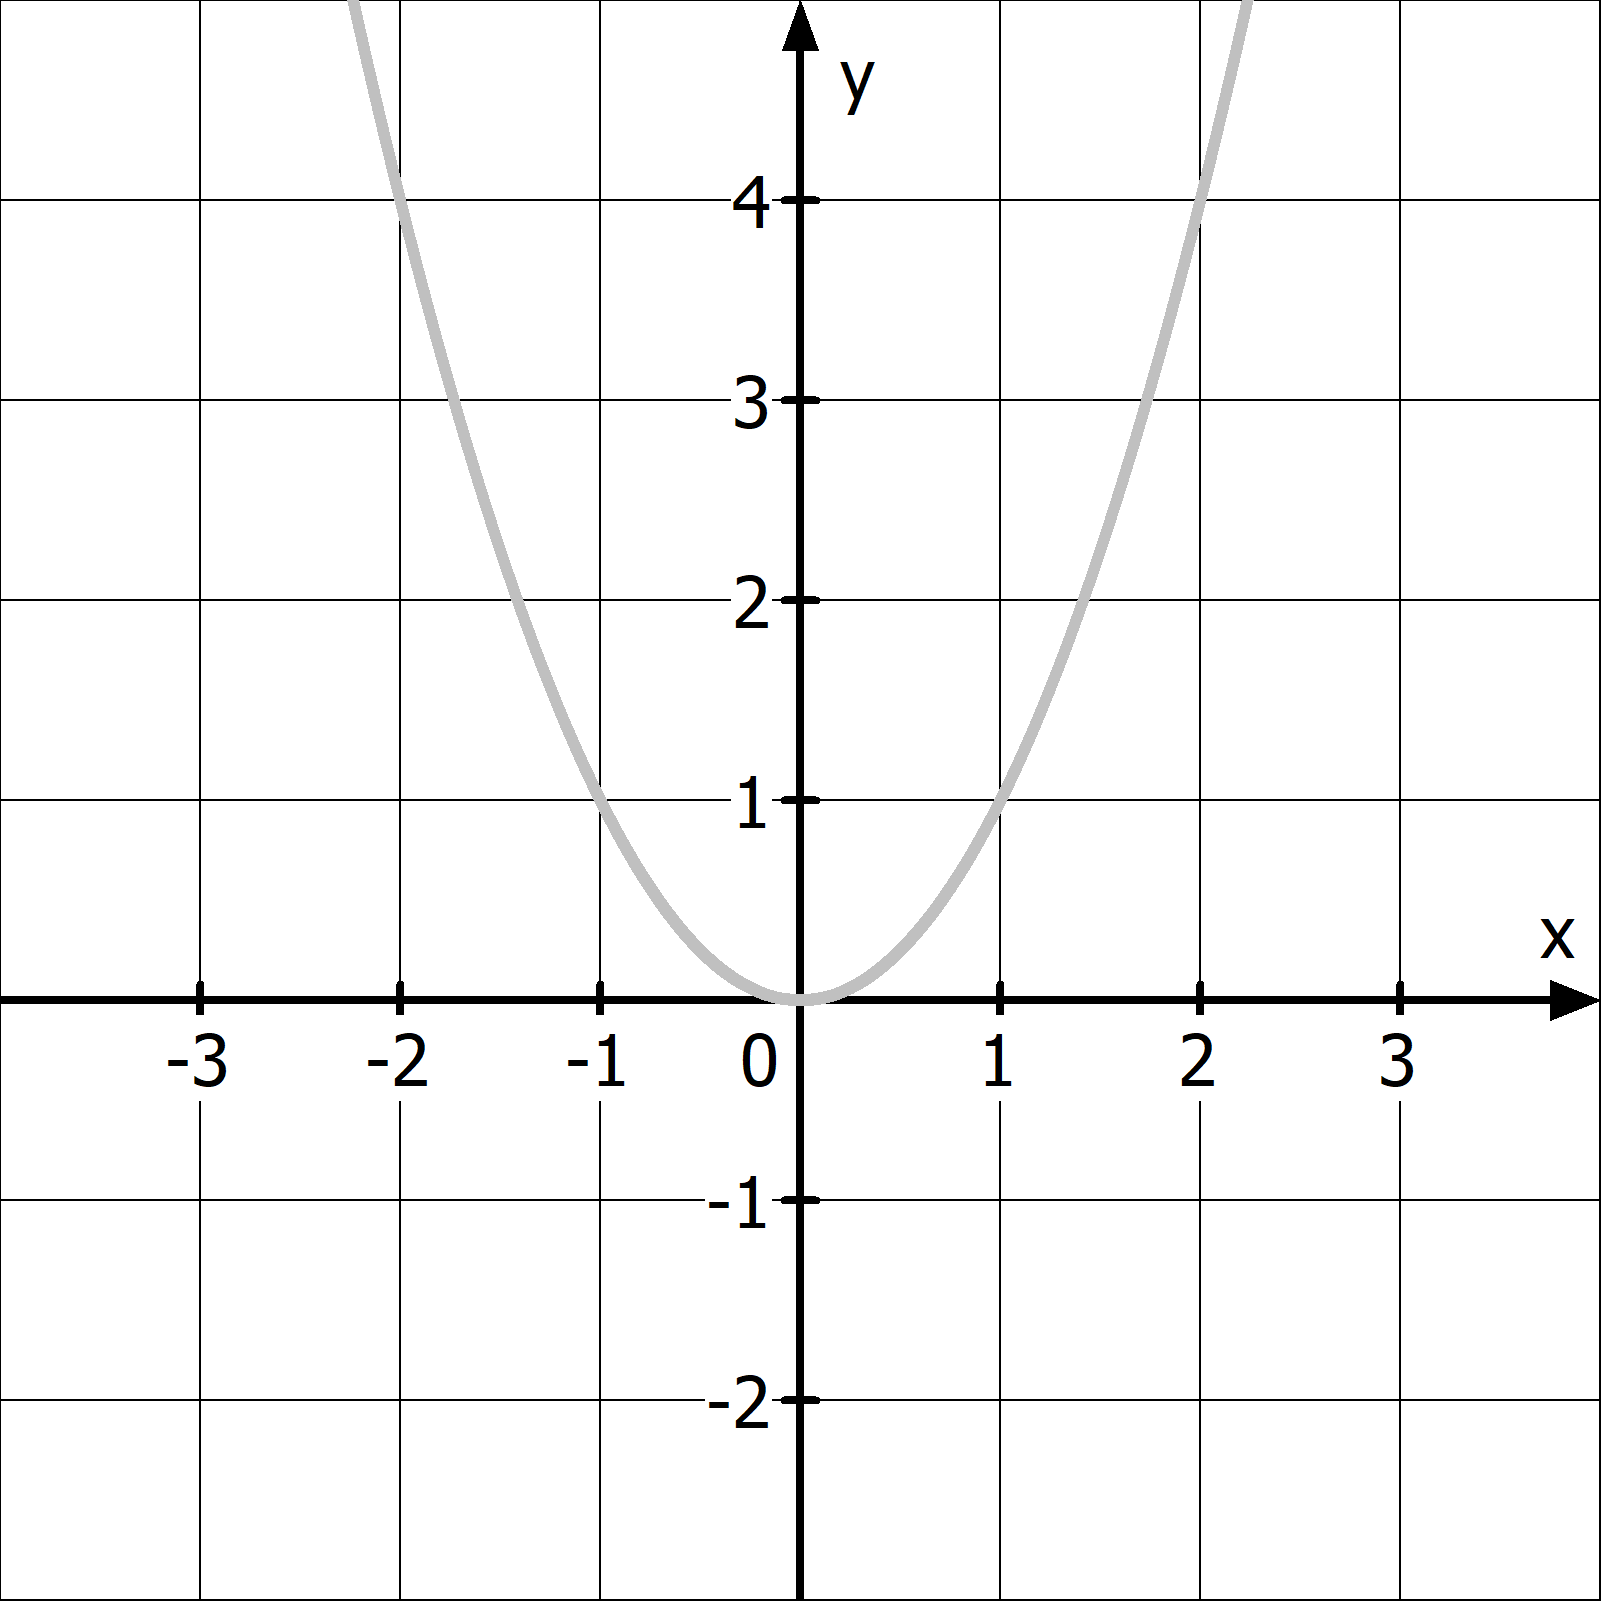
\includegraphics[width=\textwidth]{\quadFkt/pics/verschieben_empty.png}
	\end{minipage}%
	\\
\end{tabular}%
\end{minipage}
\newpage
\cohead{\Large\textbf{Verschieben in x-Richtung}}
\begin{minipage}{\textwidth}
\begin{tabular}{cc}
	\begin{minipage}{0.47\textwidth}\centering\Large
		\textcolor{loes}{Die Normalparabel wird um 2 Einheiten nach rechts verschoben.}

		\bigskip

		\textcolor{loes}{\(f(x)=\left( x-2\right)^2\)}

		\bigskip

		\textcolor{loes}{Der Scheitel liegt bei \(S\left(-2\middle\vert 0\right)\)}
	\end{minipage}%
	&
	\begin{minipage}{0.47\textwidth}
		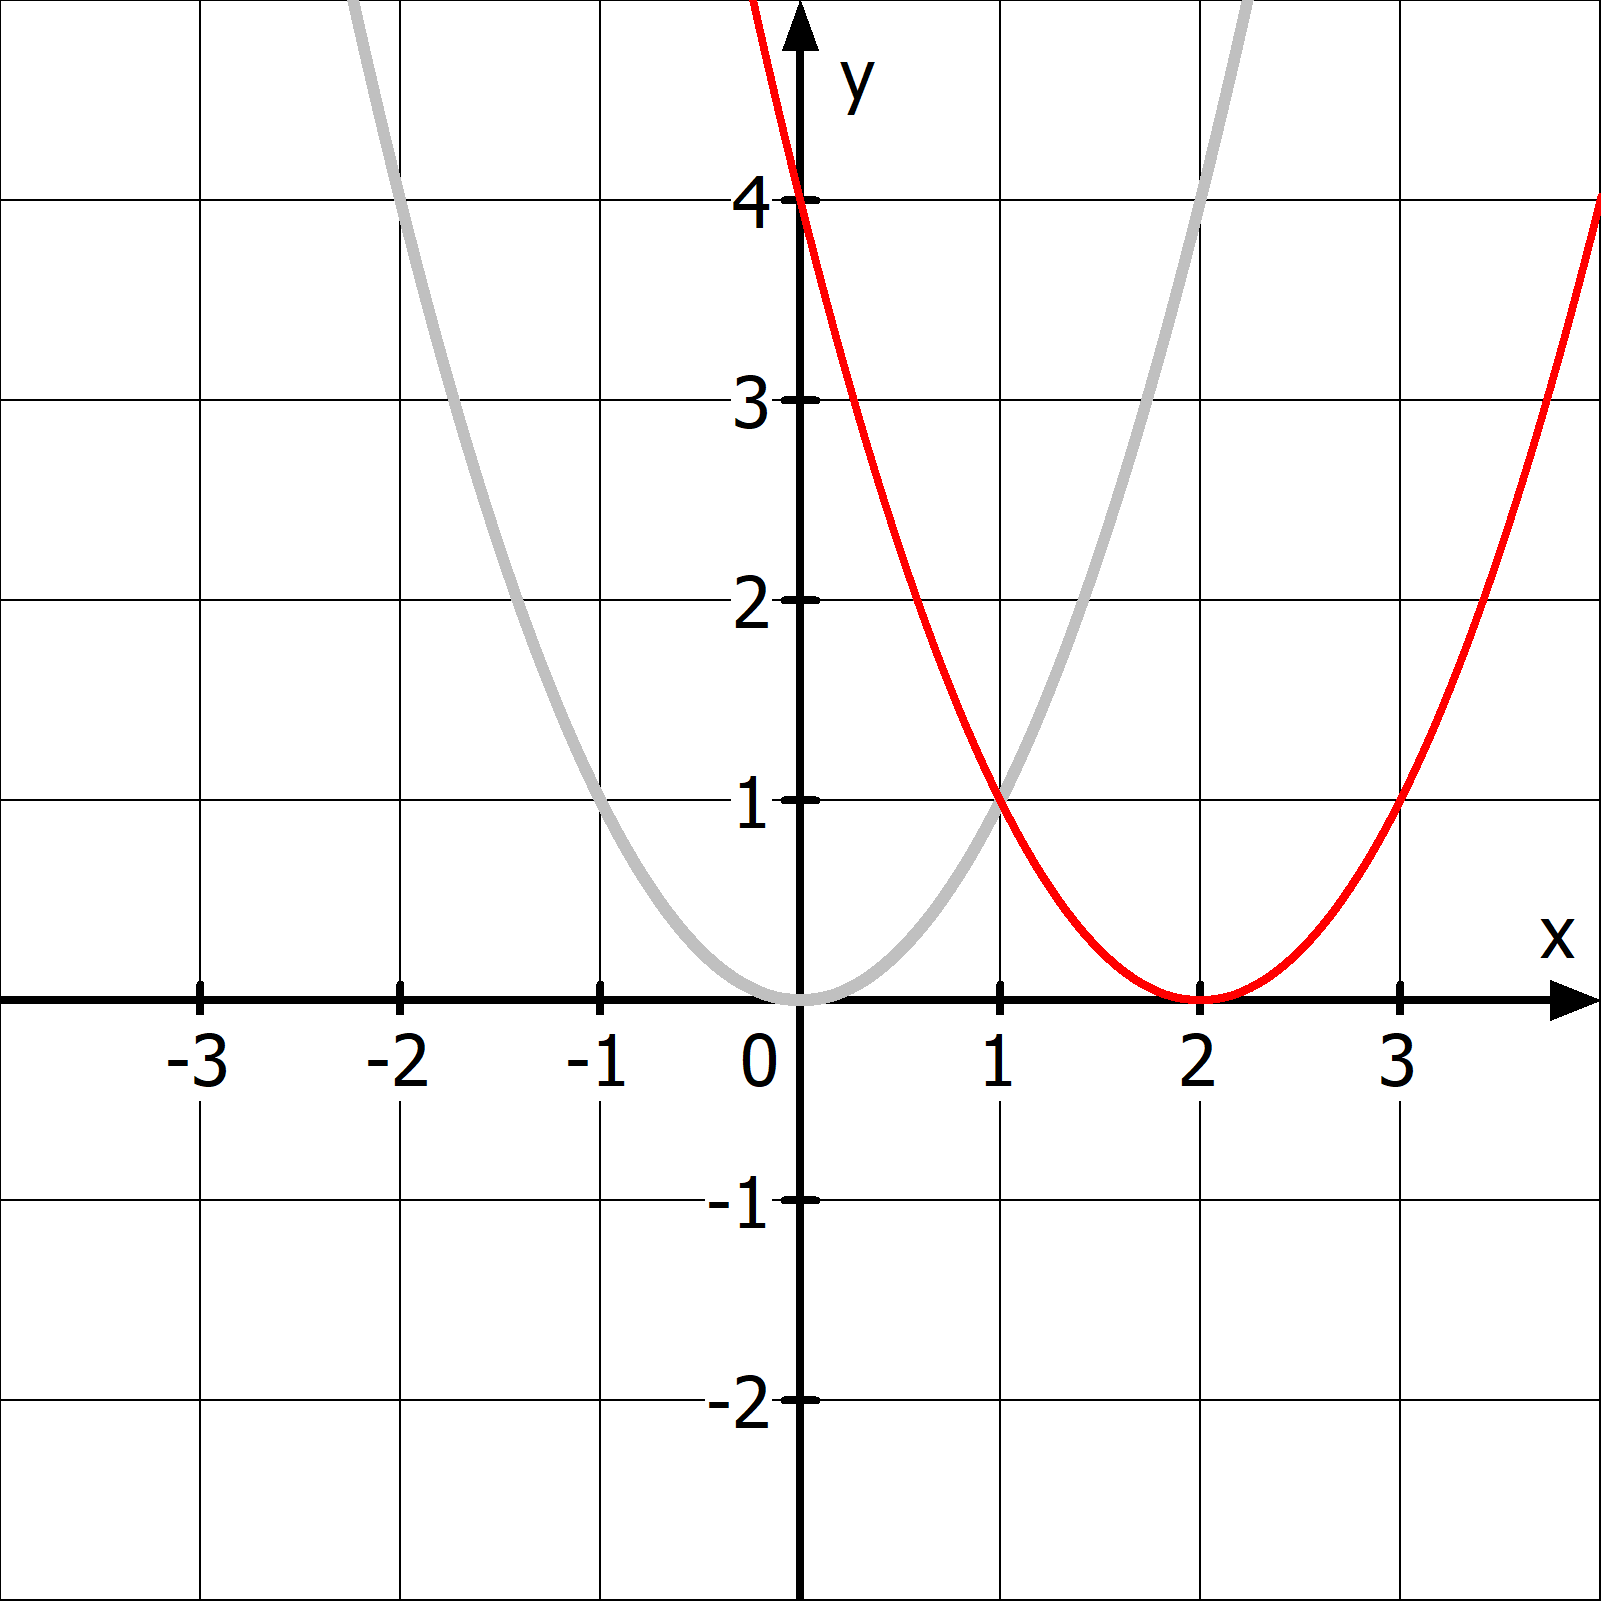
\includegraphics[width=\textwidth]{\quadFkt/pics/verschiebenX1.png}
	\end{minipage}%
	\\
	\midrule
	\begin{minipage}{0.47\textwidth}\centering\Large
		Die Normalparabel wird um 1 Einheit nach links verschoben.

		\bigskip

		\textcolor{loes}{\(f(x)=\left(x+1 \right)^2 \)}

		\bigskip

		\textcolor{loes}{Der Scheitel liegt bei \(S\left(-1\middle\vert 0\right)\)}
	\end{minipage}%
	&
	\begin{minipage}{0.47\textwidth}
		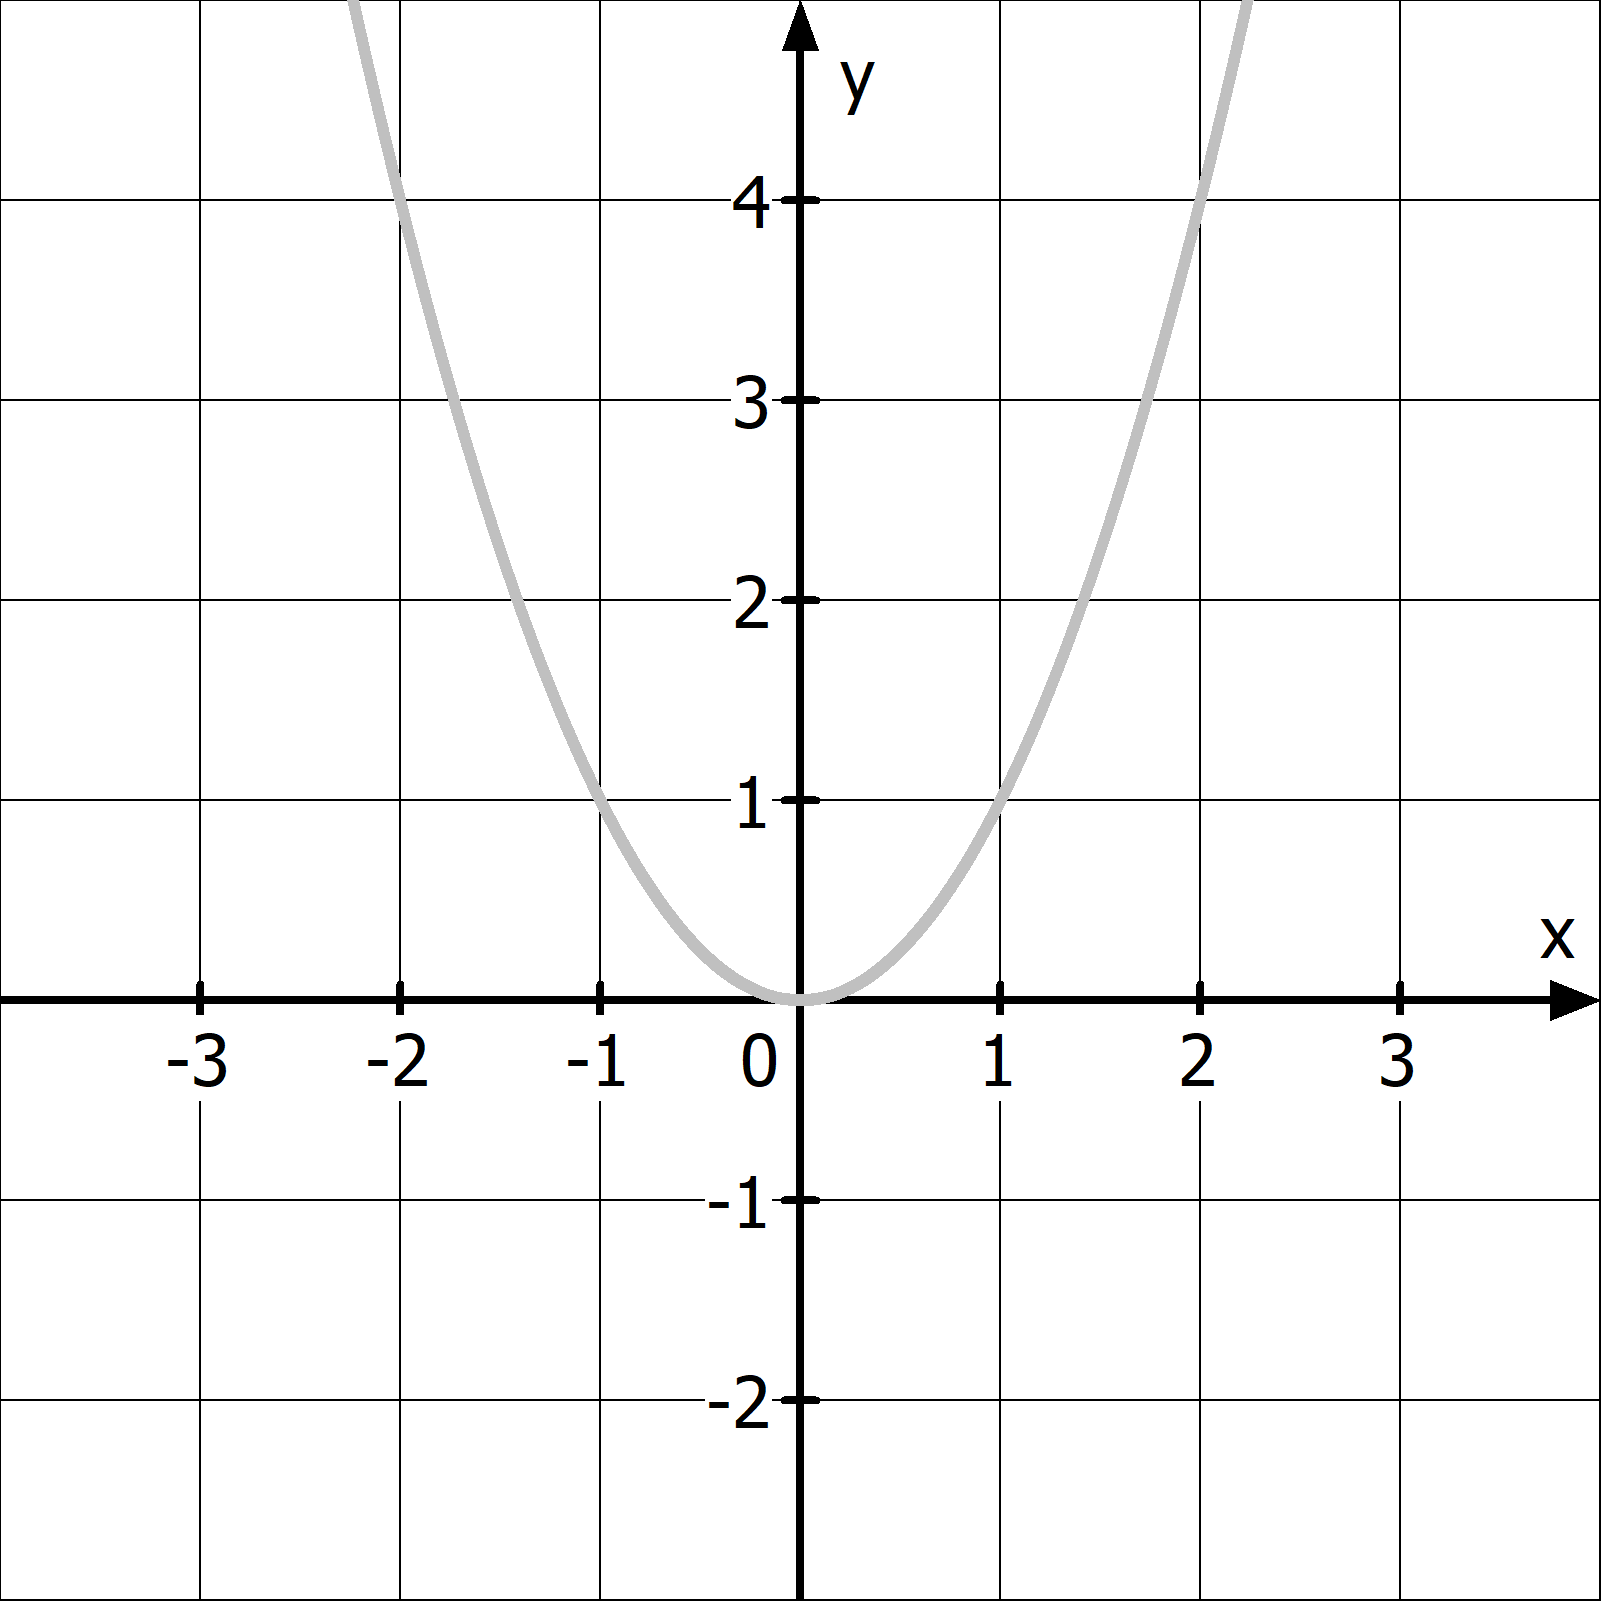
\includegraphics[width=\textwidth]{\quadFkt/pics/verschieben_empty.png}
	\end{minipage}%
	\\
	\midrule
	\begin{minipage}{0.47\textwidth}\centering\Large
		\textcolor{loes}{Die Normalparabel wird um 3 Einheiten nach rechts verschoben.}

		\bigskip

		\(f(x)=\left( x-3\right)^2\)

		\bigskip

		Der Scheitel liegt bei \(S\left(3\middle\vert 0\right)\)
	\end{minipage}%
	&
	\begin{minipage}{0.47\textwidth}
		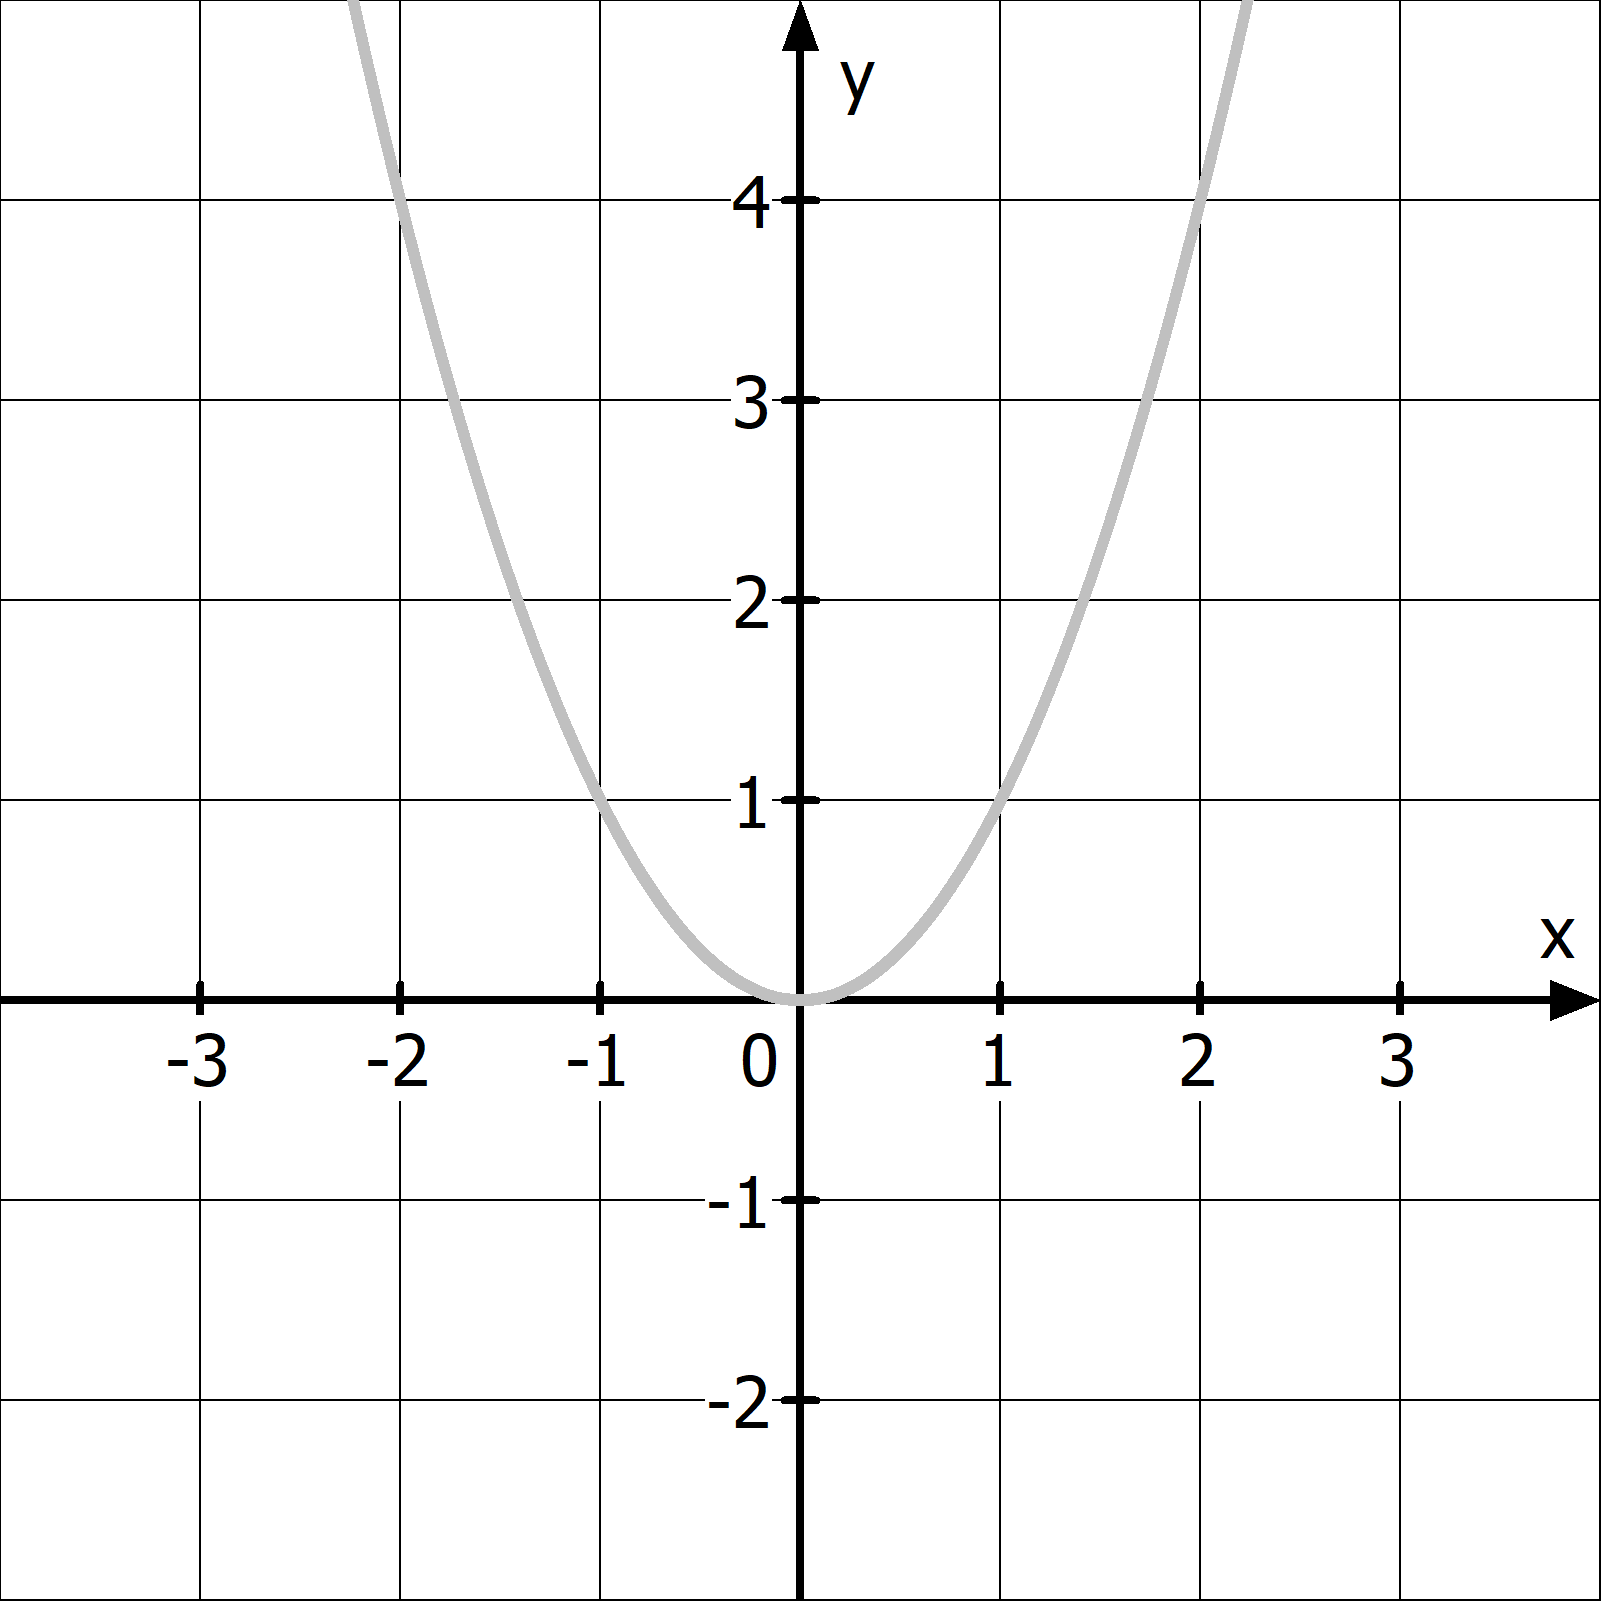
\includegraphics[width=\textwidth]{\quadFkt/pics/verschieben_empty.png}
	\end{minipage}%
	\\
\end{tabular}%
\end{minipage}\newpage
%%%%%%%%%%%%%%%%%%%%%%%%%%%%%%%%%%%%%%%%%%%%%%%%%%%%%%%%%%%%%%
\begin{Exercise}[title={Bestimme jeweils an Hand des Schaubilds die Funktionsgleichung}, label=verschiebenA1]

	\begin{minipage}{\linewidth}\centering
		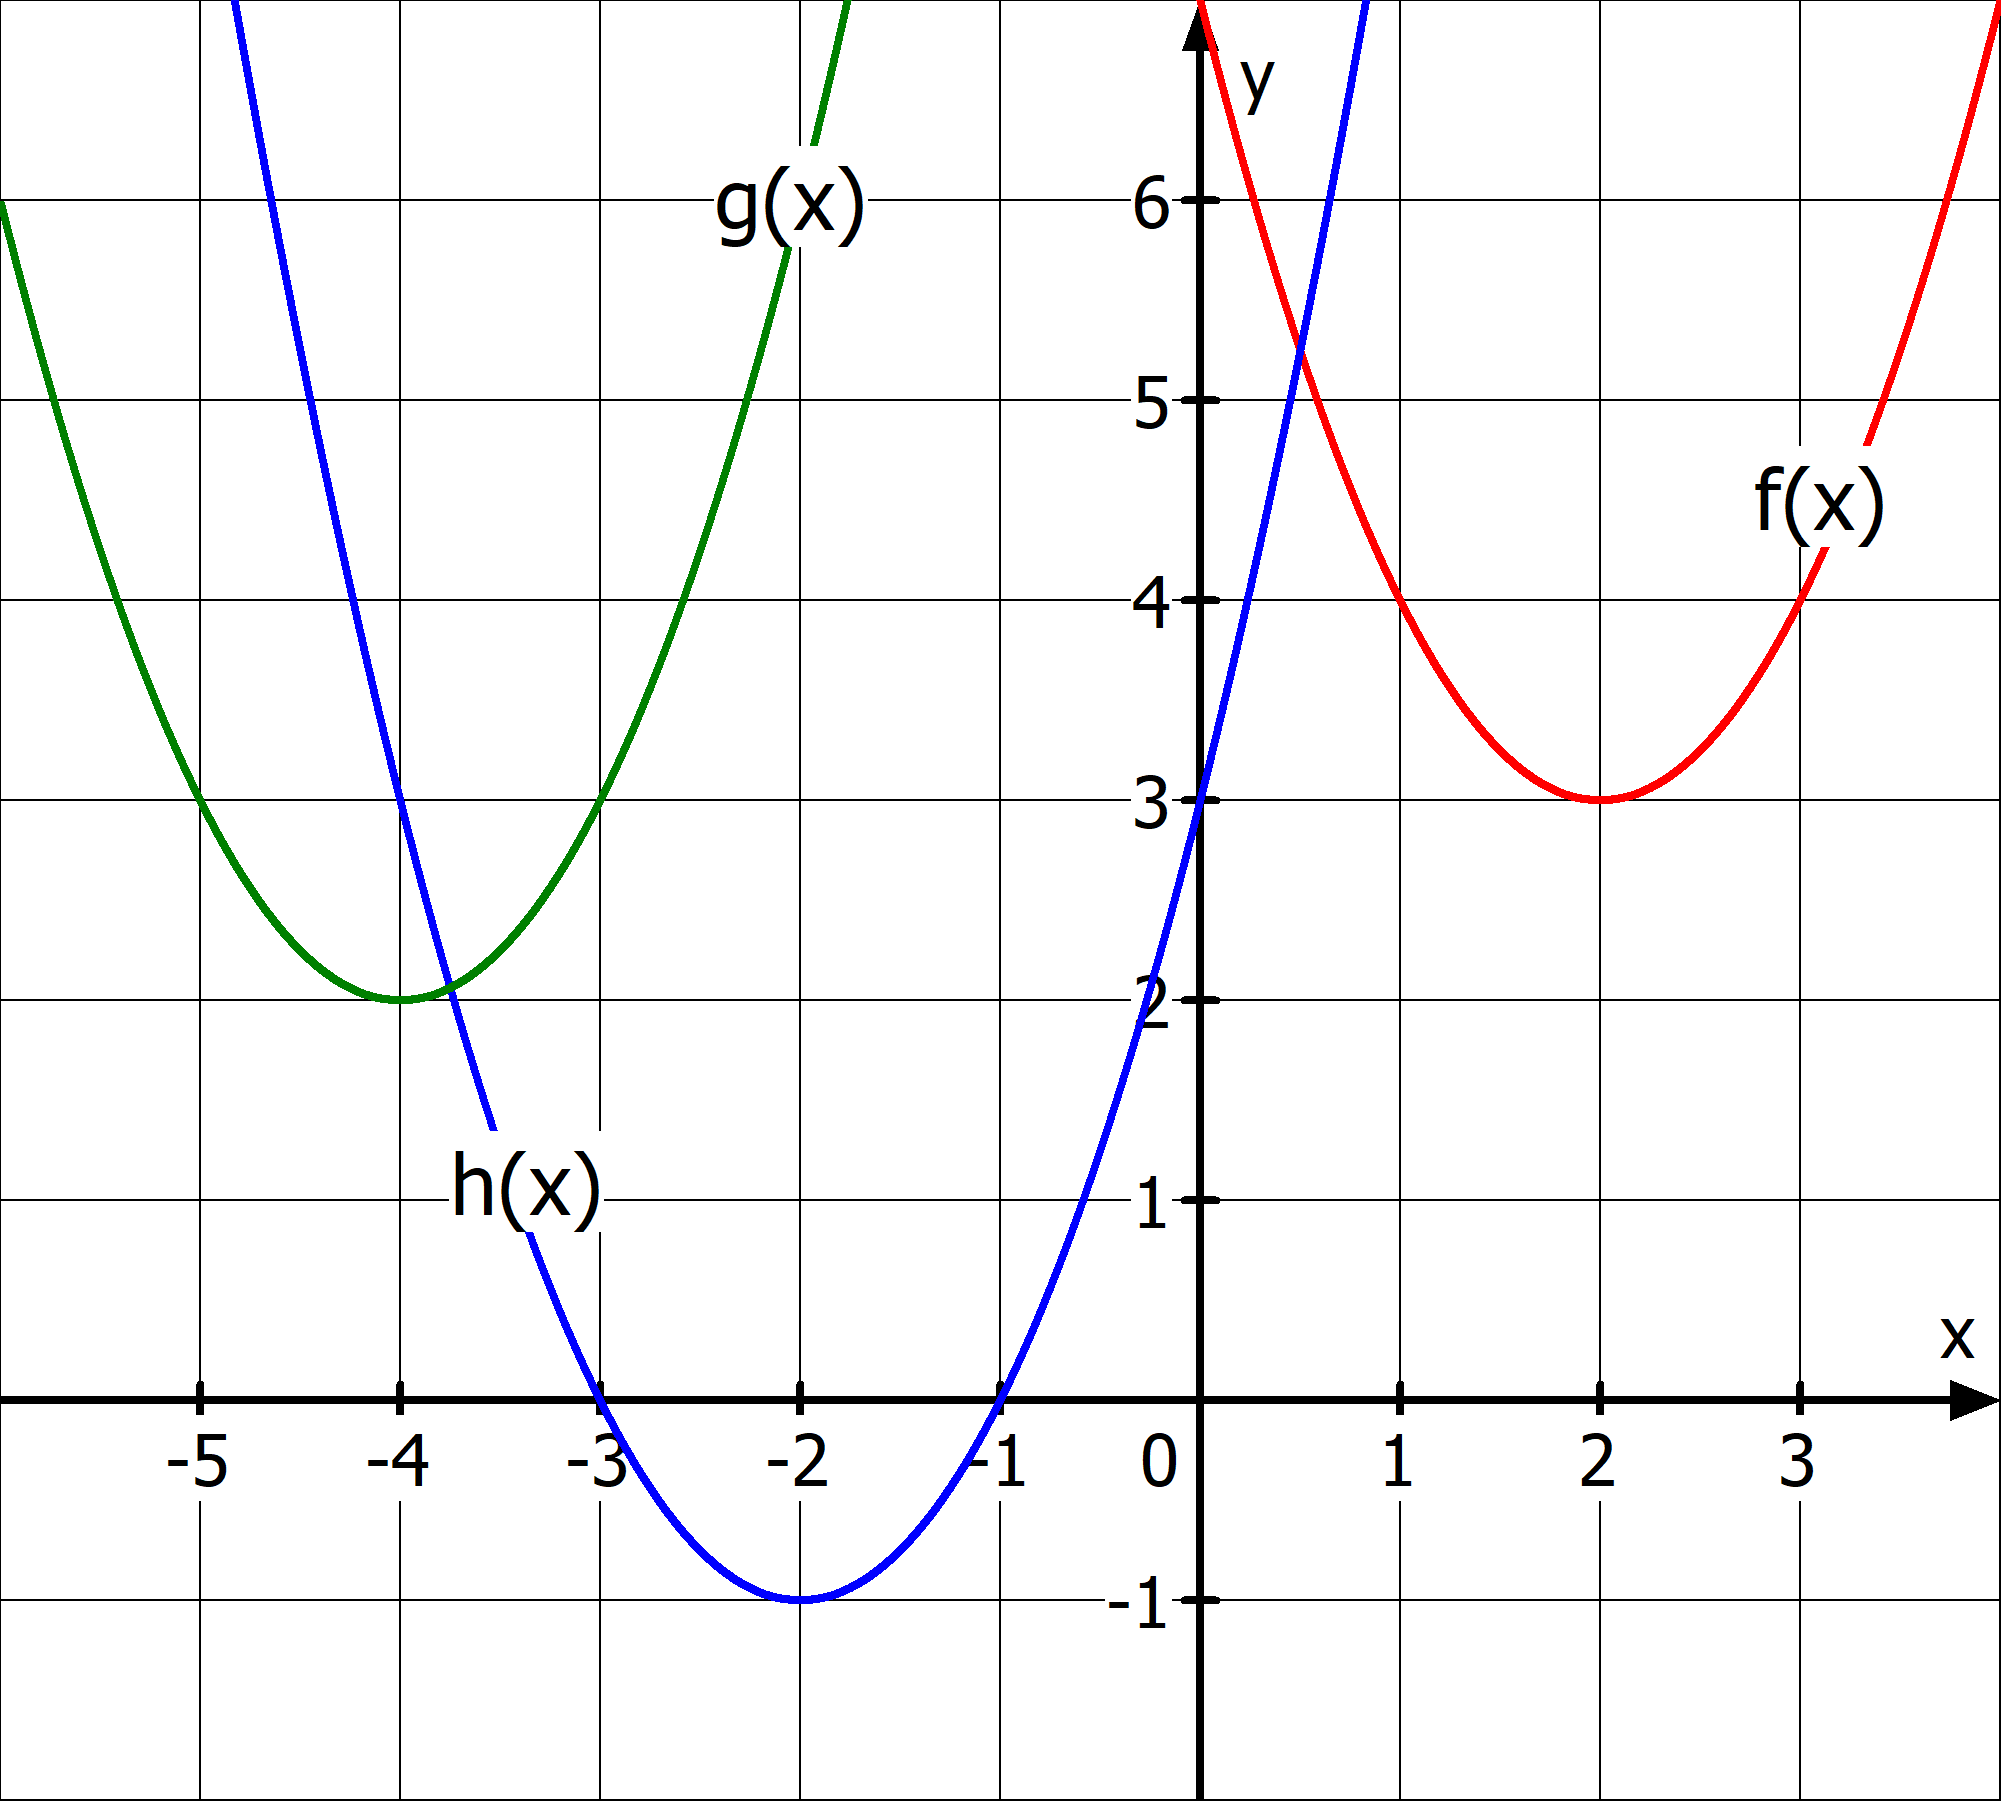
\includegraphics[width=.8\linewidth]{\quadFkt/pics/verschiebenA1.png}
	\end{minipage}%
\end{Exercise}

\begin{Exercise}[title={Stelle jeweils die Funktionsgleichung auf und skizziere das Schaubild}, label=verschiebenA2]
	\begin{enumerate}[label=\alph*)]
		\item Die Normalparabel wird um 5 Einheiten nach links und um 3 Einheiten nach unten verschoben.
		\item Die Normalparabel wird um 6 Einheiten nach rechts und um 4 Einheiten nach unten verschoben.
		\item Die Normalparabel wird um 1,5 Einheiten nach links und um 2,5 Einheiten nach oben verschoben.
	\end{enumerate}
\end{Exercise}
\begin{Exercise}[title={Beschreibe wie man die Normalparabel verschieben muss und skizziere das Schaubild}, label=verschiebenA3]
	\begin{enumerate}[label=\alph*)]
		\item \(f(x)=(x-3)^2-4\) \quad b) \(g(x)=(x+4)^2+3\) \quad c) \(h(x)=\left(x-\tfrac{3}{2}\right)^2+\tfrac{5}{2}\)
	\end{enumerate}
\end{Exercise}
\begin{Exercise}[title={Stelle die Funktionsgleichung auf}, label=verschiebenA4]
	\begin{enumerate}[label=\alph*)]
		\item Das Schaubild von \(f(x)=(x-2)^2+1\) wird um 3 Einheiten nach links und 4 Einheiten nach oben verschoben.
		\item Das Schaubild von \(g(x)=(x+3)^2-2\) wird um 4 Einheiten nach rechts und 2 Einheiten nach oben verschoben.
	\end{enumerate}
\end{Exercise}\newpage
\begin{Answer}[ref=verschiebenA1]\\
	\begin{minipage}{\linewidth}\centering
		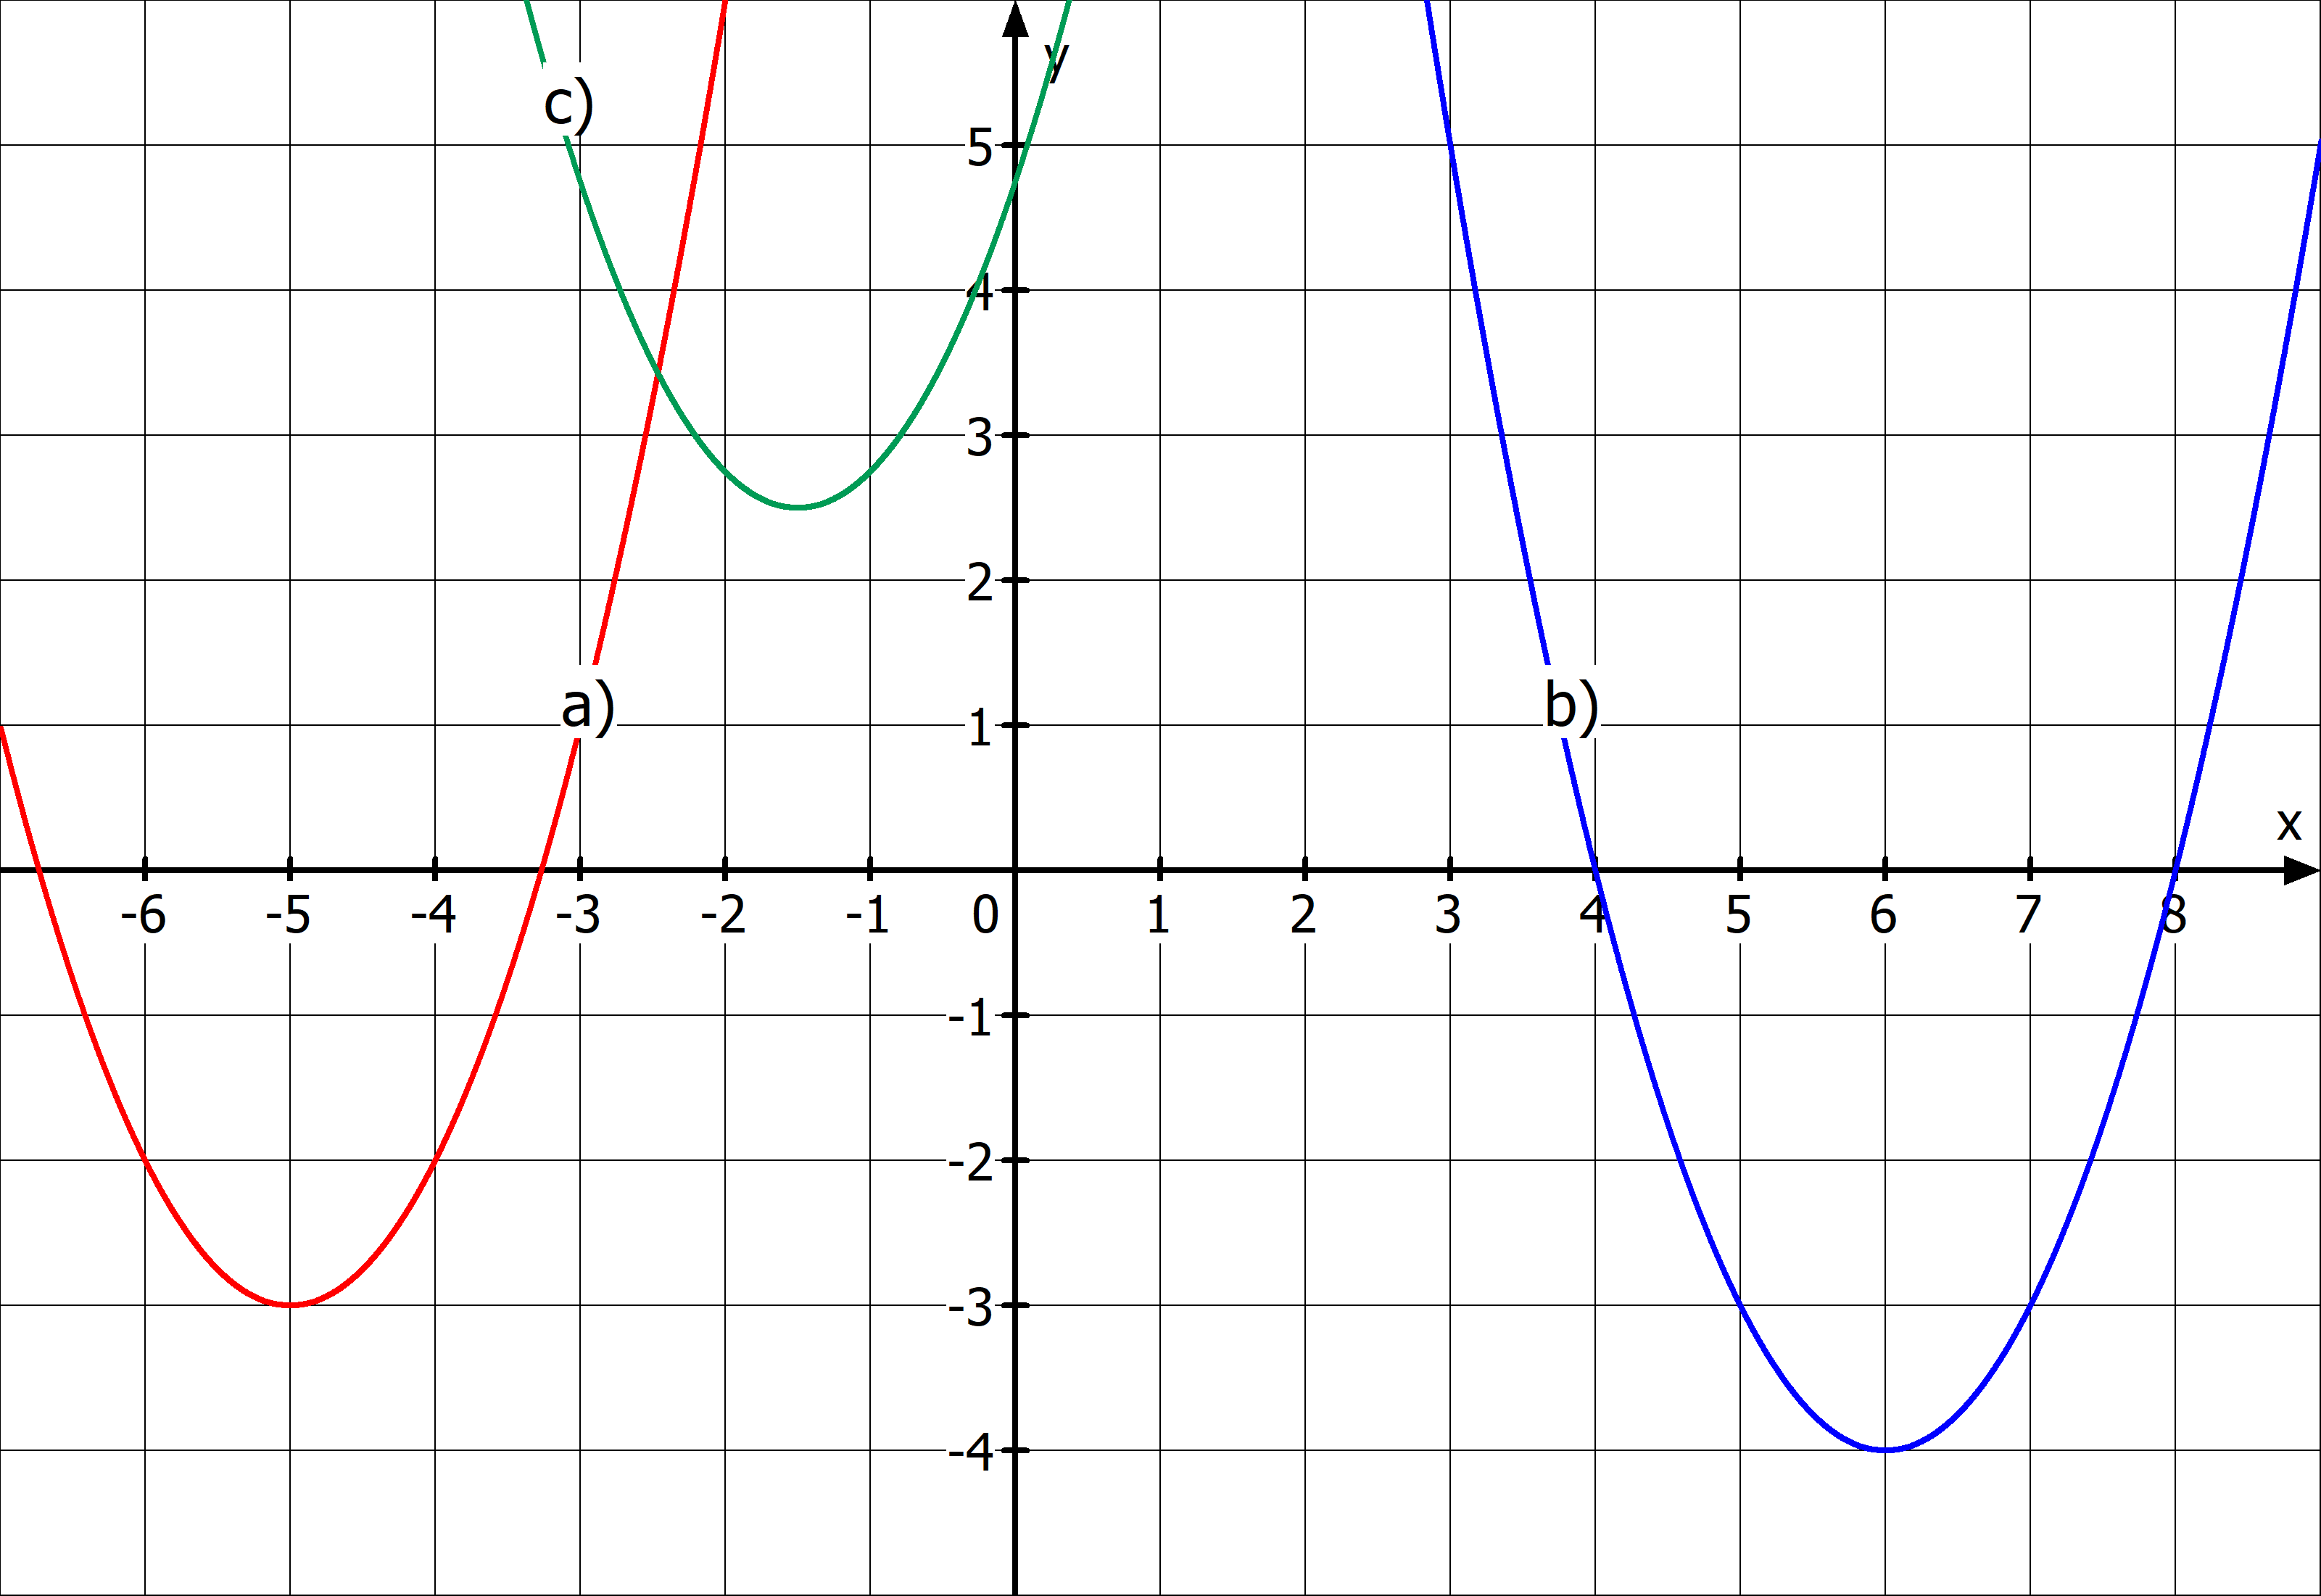
\includegraphics[width=.7\linewidth]{\quadFkt/pics/verschiebenA2.png}
	\end{minipage}\vspace{.1cm}
	\begin{enumerate}[label=\alph*)]
		\item \(f(x)=\left(x-2\right)^2+3\) \quad b) \(g(x)=\left(x+4\right)^2+2\) \quad c) \(h(x)=\left(x+2\right)^2-1\)
	\end{enumerate}
\end{Answer}

\begin{Answer}[ref=verschiebenA2]
	\begin{enumerate}[label=\alph*)]
		\item \(f(x)=\left(x+5\right)^2-3\) \quad b) \(g(x)=\left(x-6\right)^2-4\) \quad c) \(h(x)=\left(x+1,5\right)^2+2,5\)
	\end{enumerate}
\end{Answer}


\begin{Answer}[ref=verschiebenA3]\\
	\begin{minipage}{\linewidth}\centering
		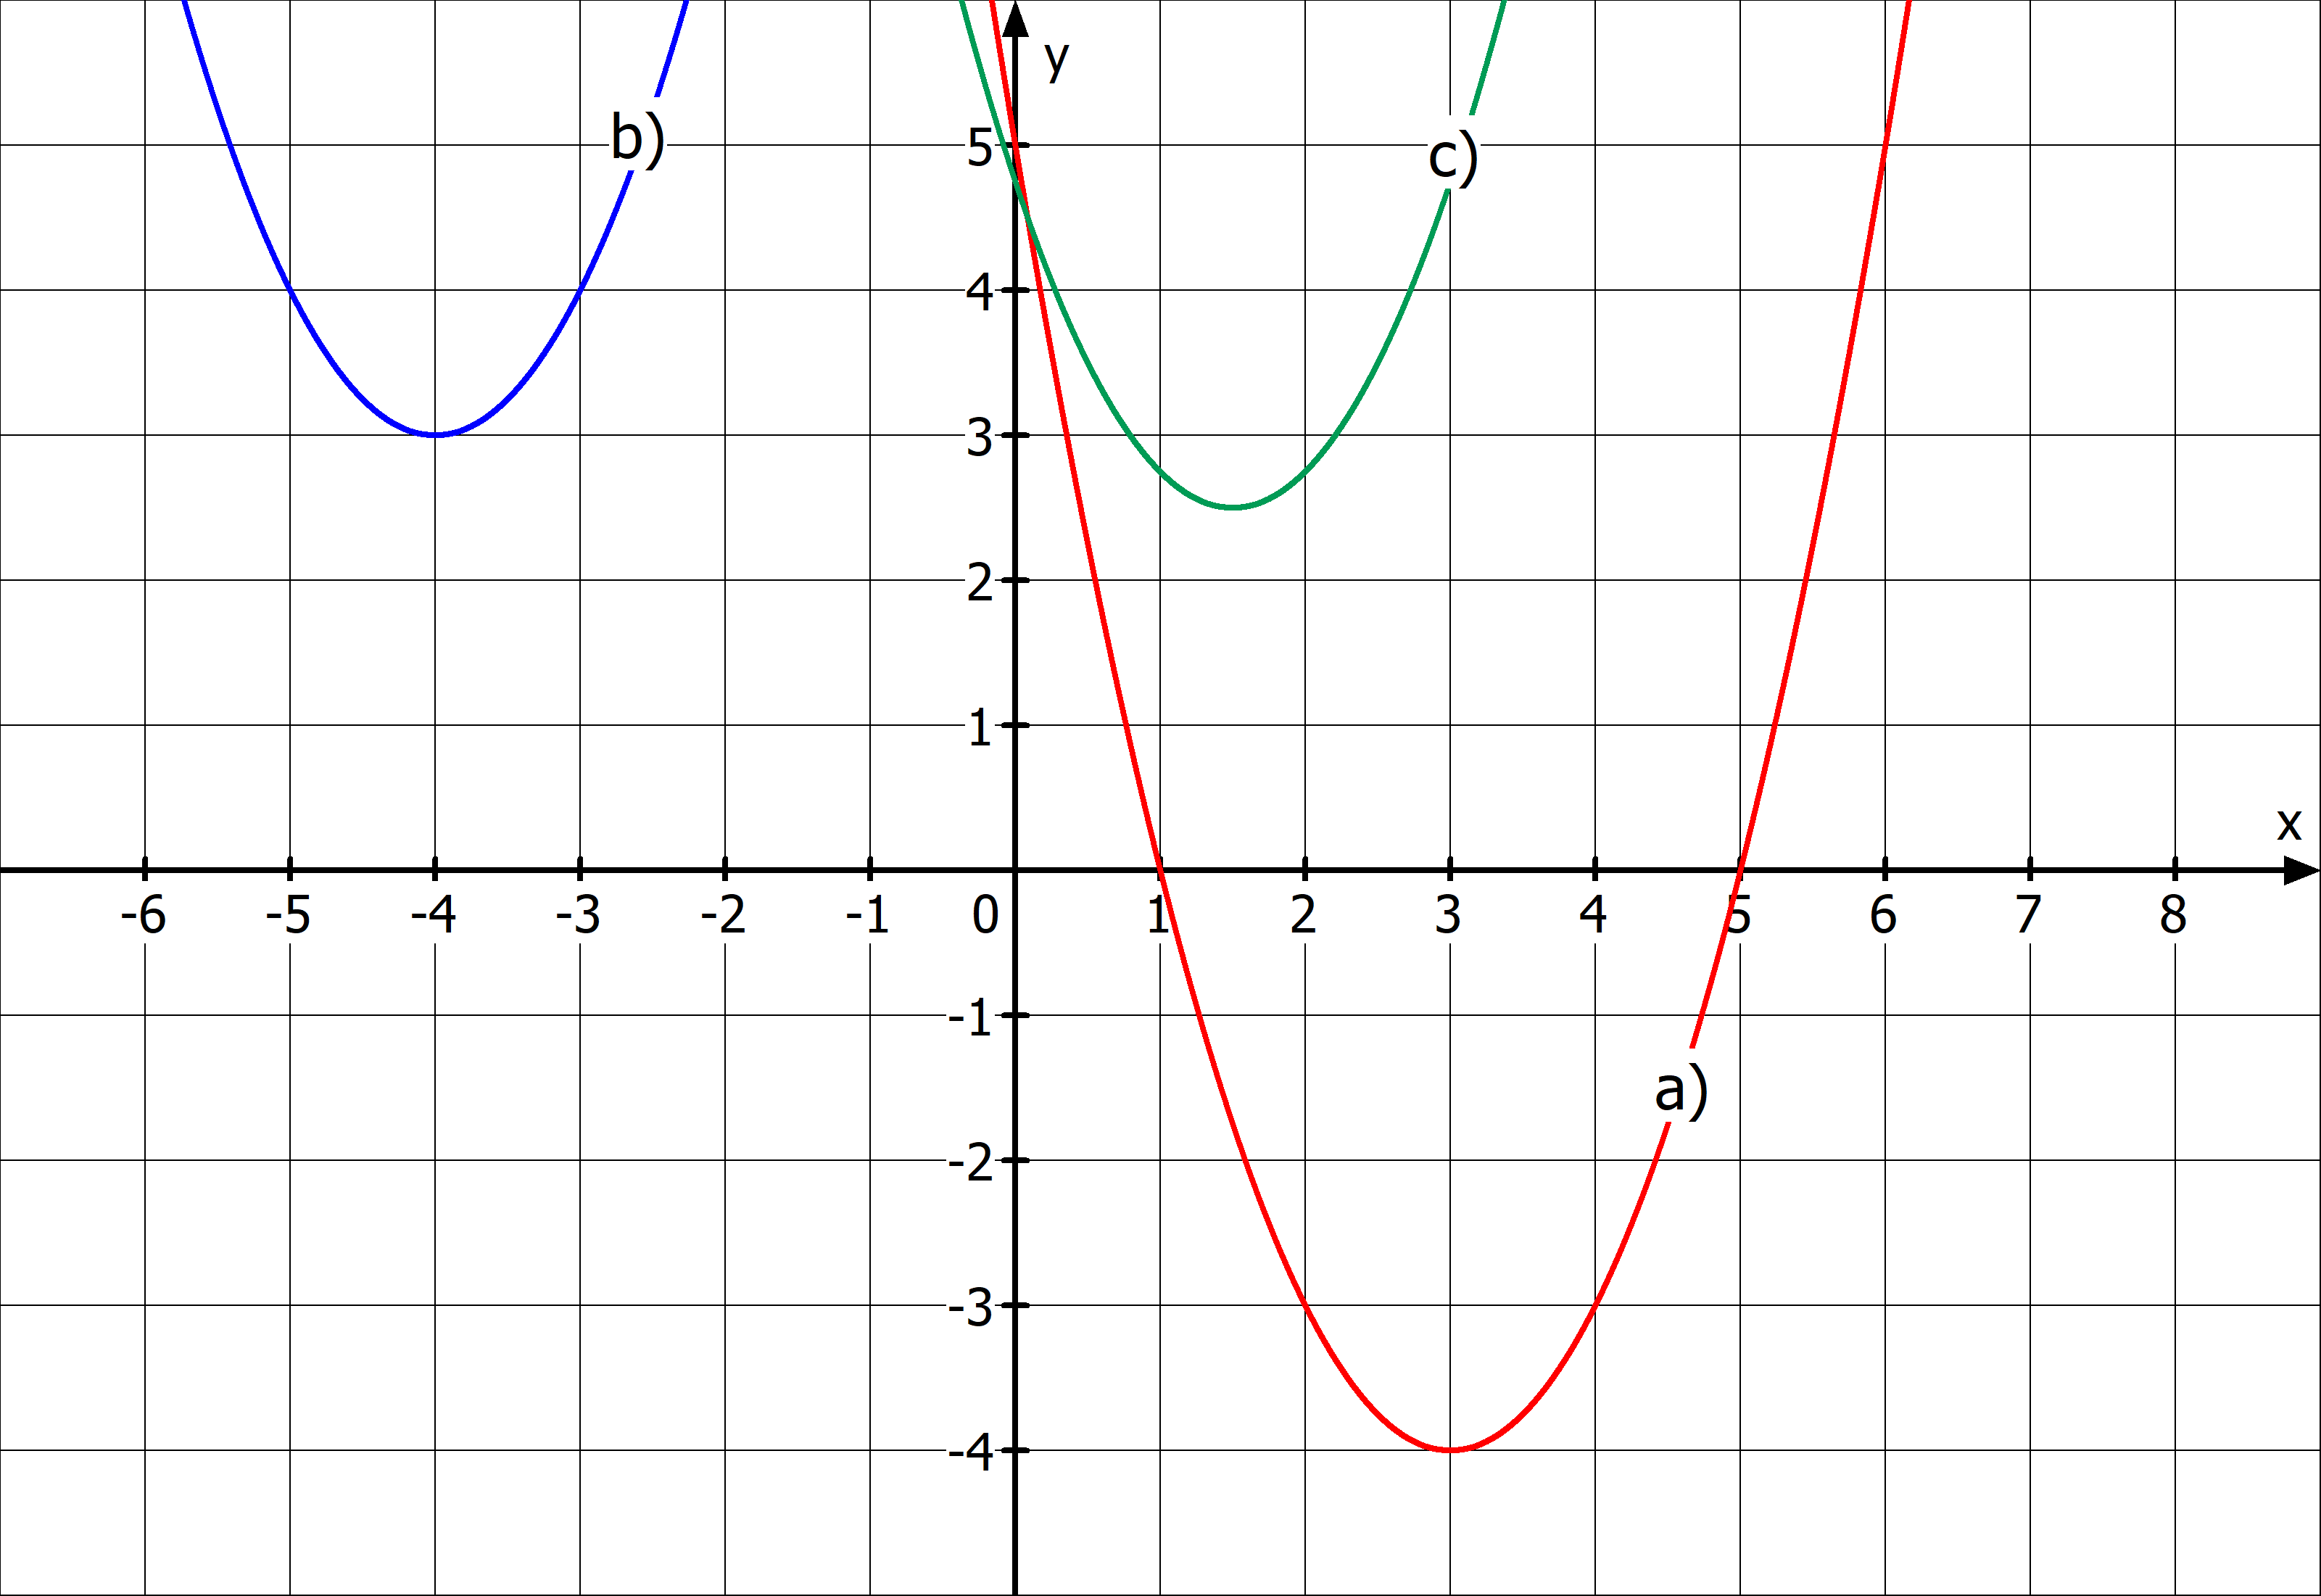
\includegraphics[width=.7\linewidth]{\quadFkt/pics/verschiebenA3.png}
	\end{minipage}\vspace{.1cm}
	\begin{enumerate}[label=\alph*)]
		\item Die Normalparabel wird um 3 Einheiten nach rechts und 4 Einheiten nach unten verschoben.
		\item Die Normalparabel wird um 4 Einheiten nach links und 3 Einheiten nach oben verschoben.
		\item Die Normalparabel wird um 1,5 Einheiten nach rechts und 2,5 Einheiten nach oben verschoben.
	\end{enumerate}
\end{Answer}
\begin{Answer}[ref=verschiebenA4]
	\begin{enumerate}[label=\alph*)]
		\item \(f_v(x)=(x+1)^2+5\) \quad b) \(g_v(x)=(x-1)^2\)
	\end{enumerate}
\end{Answer}\newpage
%%%%%%%%%%%%%%%%%%%%%%%%%%%%%%%%%%%%%%%%
\cohead{\Large\textbf{Strecken und Stauchen}}
\begin{tabular}{cc}
	\begin{minipage}{0.47\textwidth}\centering\Large
		\textcolor{loes}{Die Normalparabel wird mit dem Faktor \(2\) gestreckt.}

		\bigskip

		\textcolor{loes}{\(f(x)=2x^2\)}
	\end{minipage}
	&
	\begin{minipage}{0.47\textwidth}\centering
		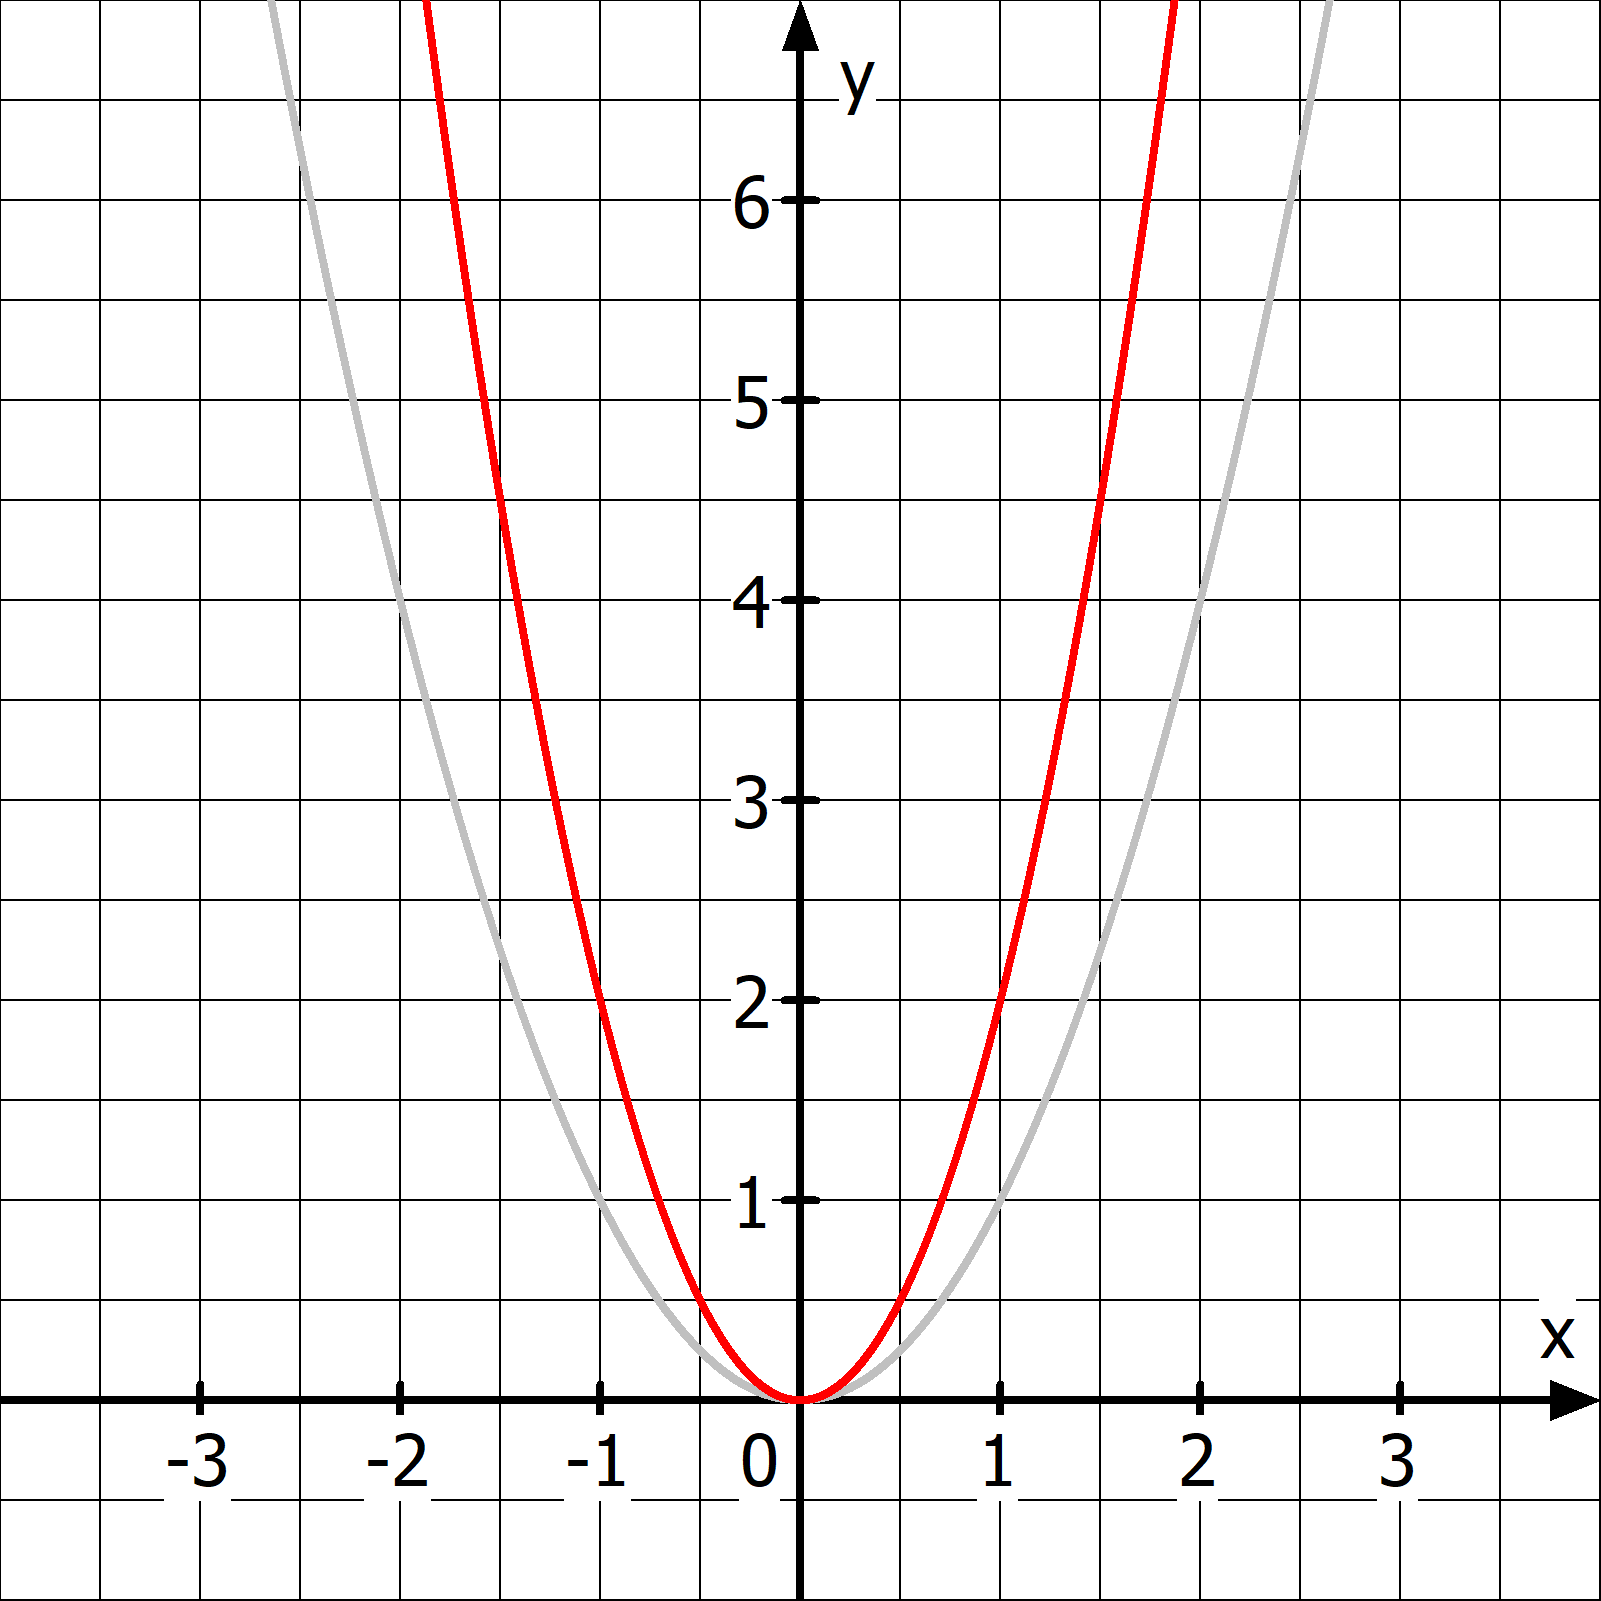
\includegraphics[width=.95\textwidth]{\quadFkt/pics/strecken1.png}
	\end{minipage} \\
	\midrule
	\begin{minipage}{0.47\textwidth}\centering\Large
		Die Normalparabel wird mit dem Faktor \(2\) gestaucht oder mit dem Faktor \(\tfrac{1}{2}\) gestreckt.

		\bigskip

		\textcolor{loes}{\(f(x)=\dfrac{1}{2}x^2\)}
	\end{minipage}
	&
	\begin{minipage}{0.47\textwidth}\centering
		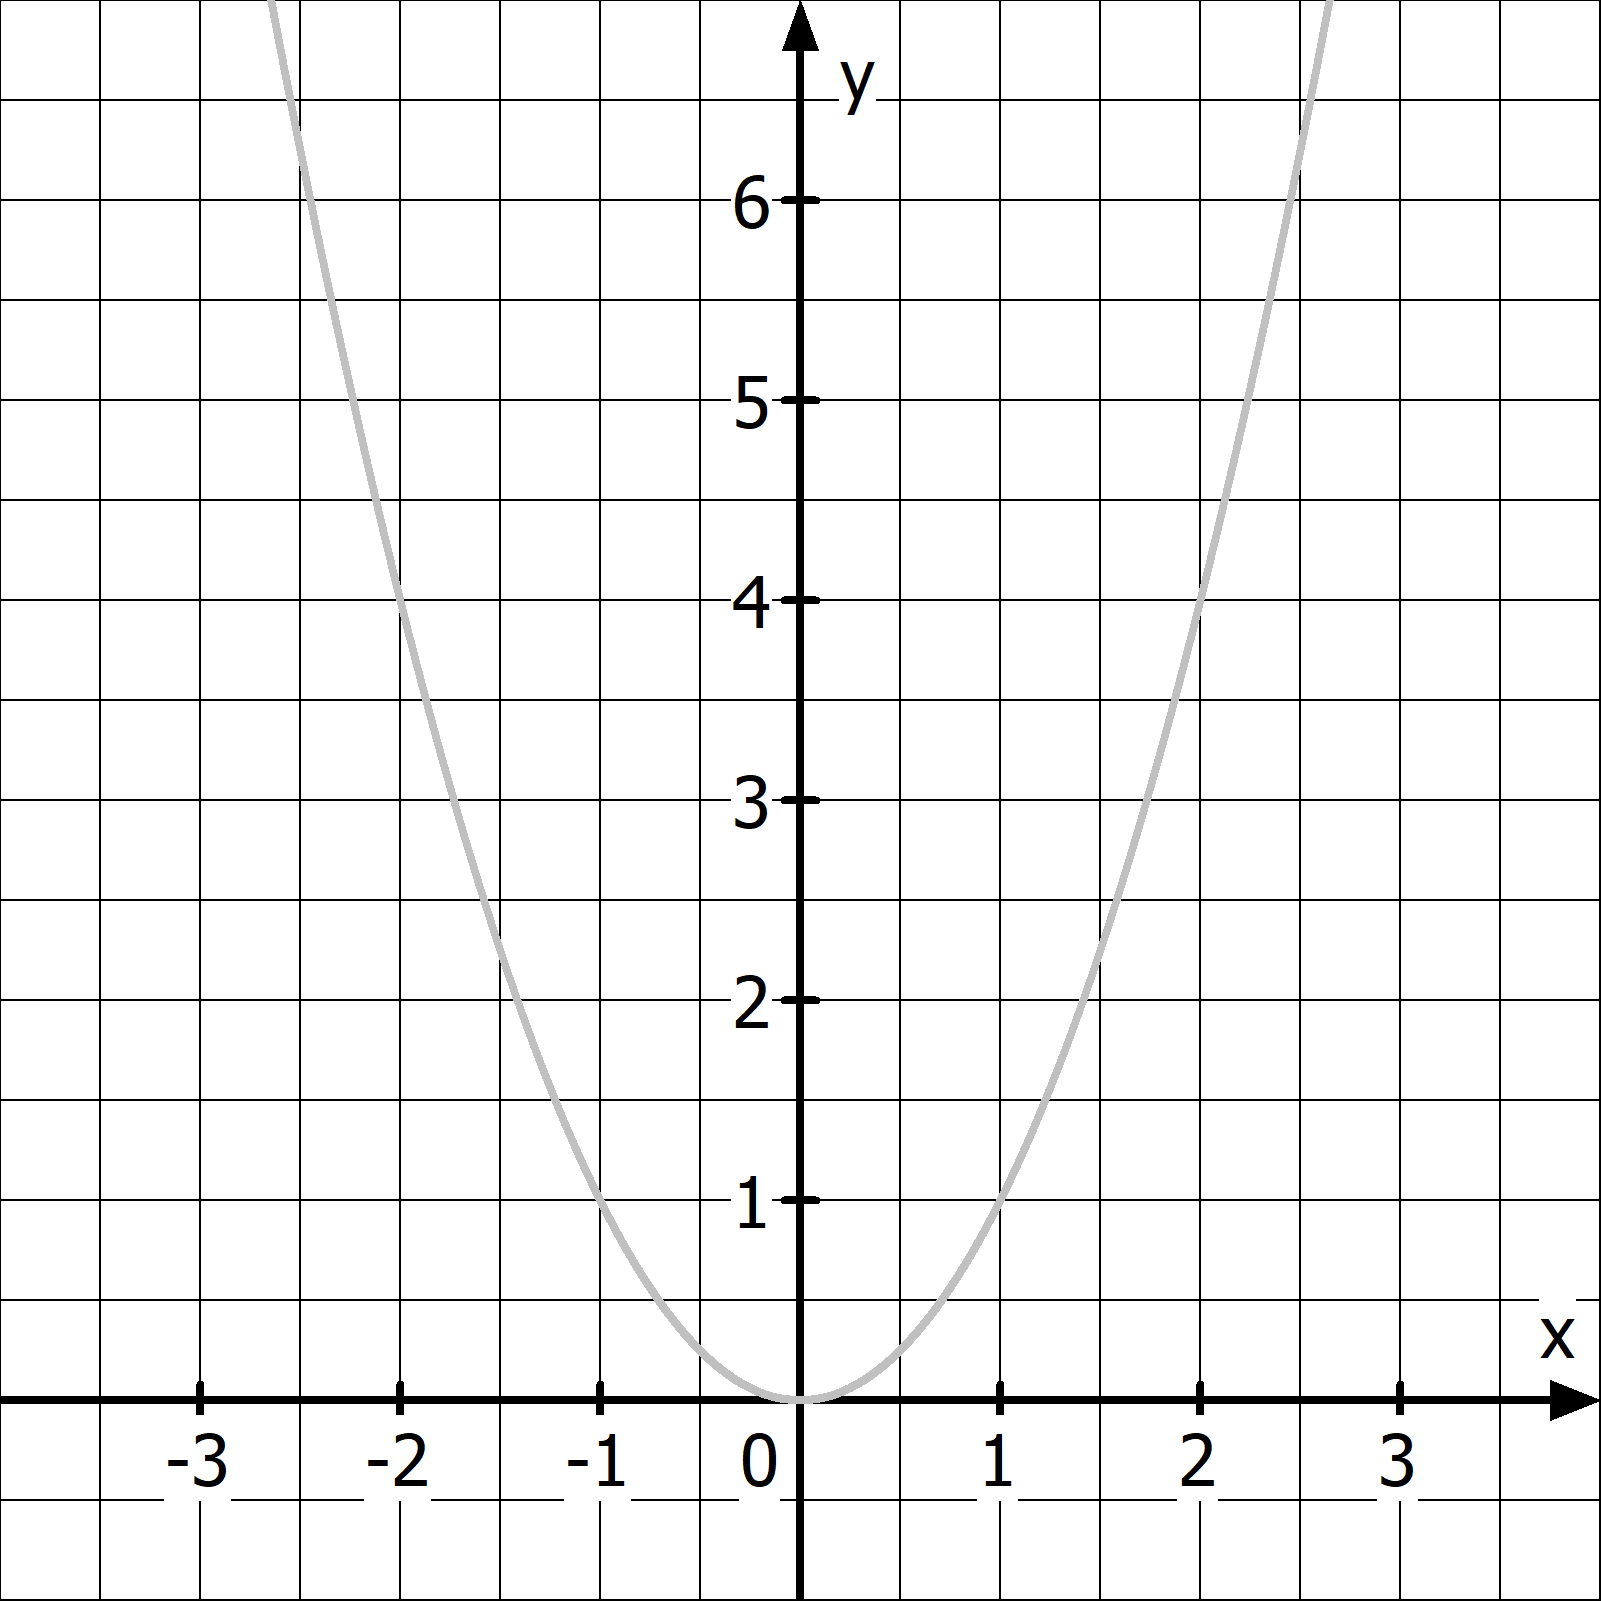
\includegraphics[width=.95\textwidth]{\quadFkt/pics/strecken2.png}
	\end{minipage} \\
	\midrule
	\begin{minipage}{0.47\textwidth}\centering\Large
		\textcolor{loes}{Die Normalparabel wird am Scheitel nach unten geklappt und mit dem Faktor \(3\) gestaucht oder mit dem Faktor \(\tfrac{1}{3}\) gestreckt.}

		\bigskip

		\(f(x)=-\dfrac{1}{3}x^2\)
	\end{minipage}
	&
	\begin{minipage}{0.47\textwidth}\centering
		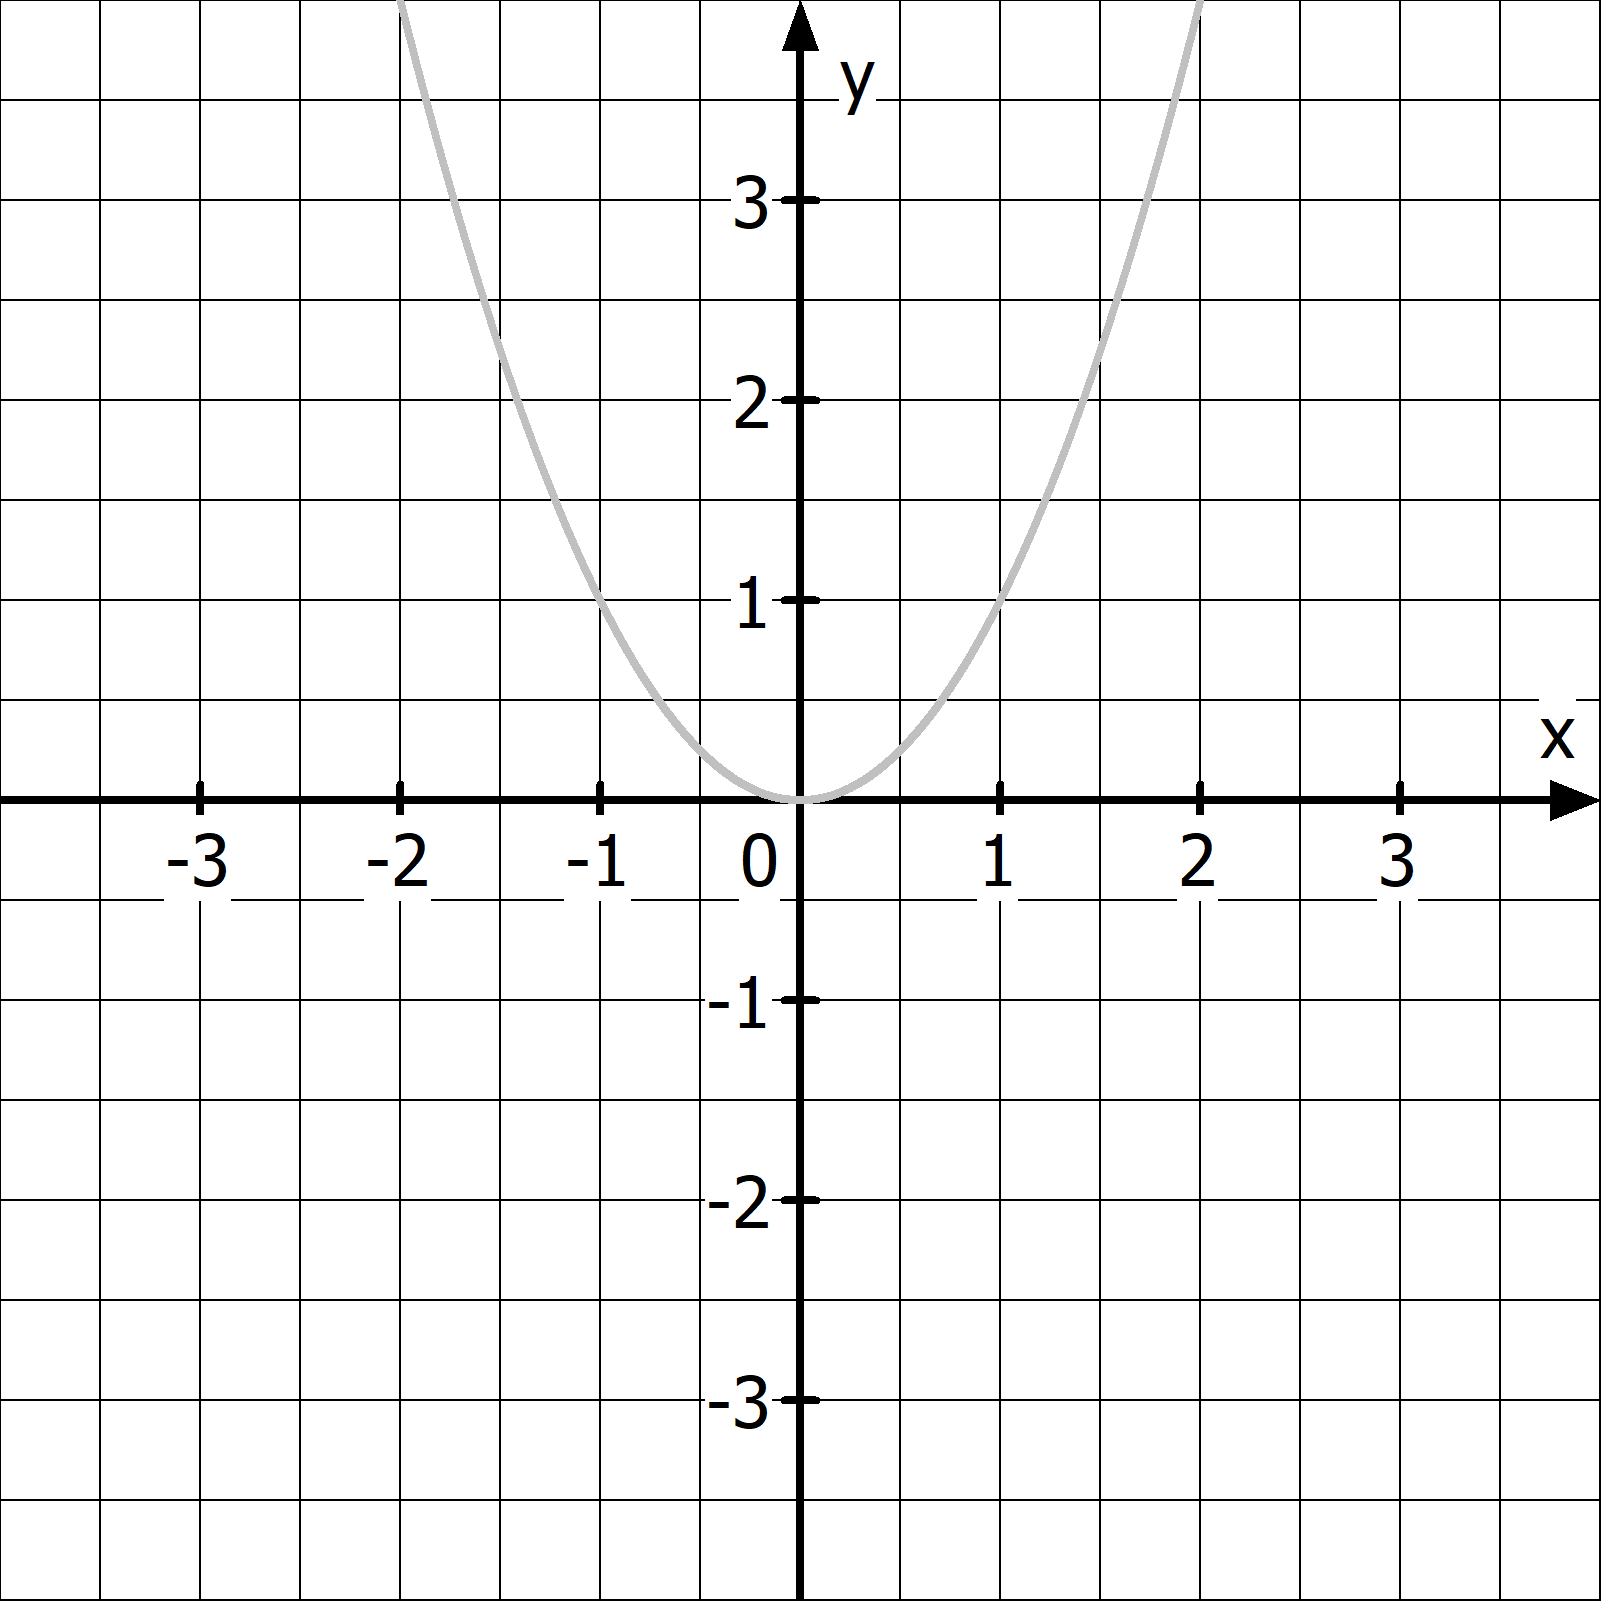
\includegraphics[width=.95\textwidth]{\quadFkt/pics/strecken3.png}
	\end{minipage} \\
\end{tabular}\newpage
%%%%%%%%%%%%%%%%%%%%%%%%%%%%%%%%%%%%%%%%%%%%%%%

\begin{Exercise}[title={Bestimme jeweils an Hand des Schaubilds die Funktionsgleichung}, label=scheitelformA1]

	\begin{minipage}{\linewidth}\centering
		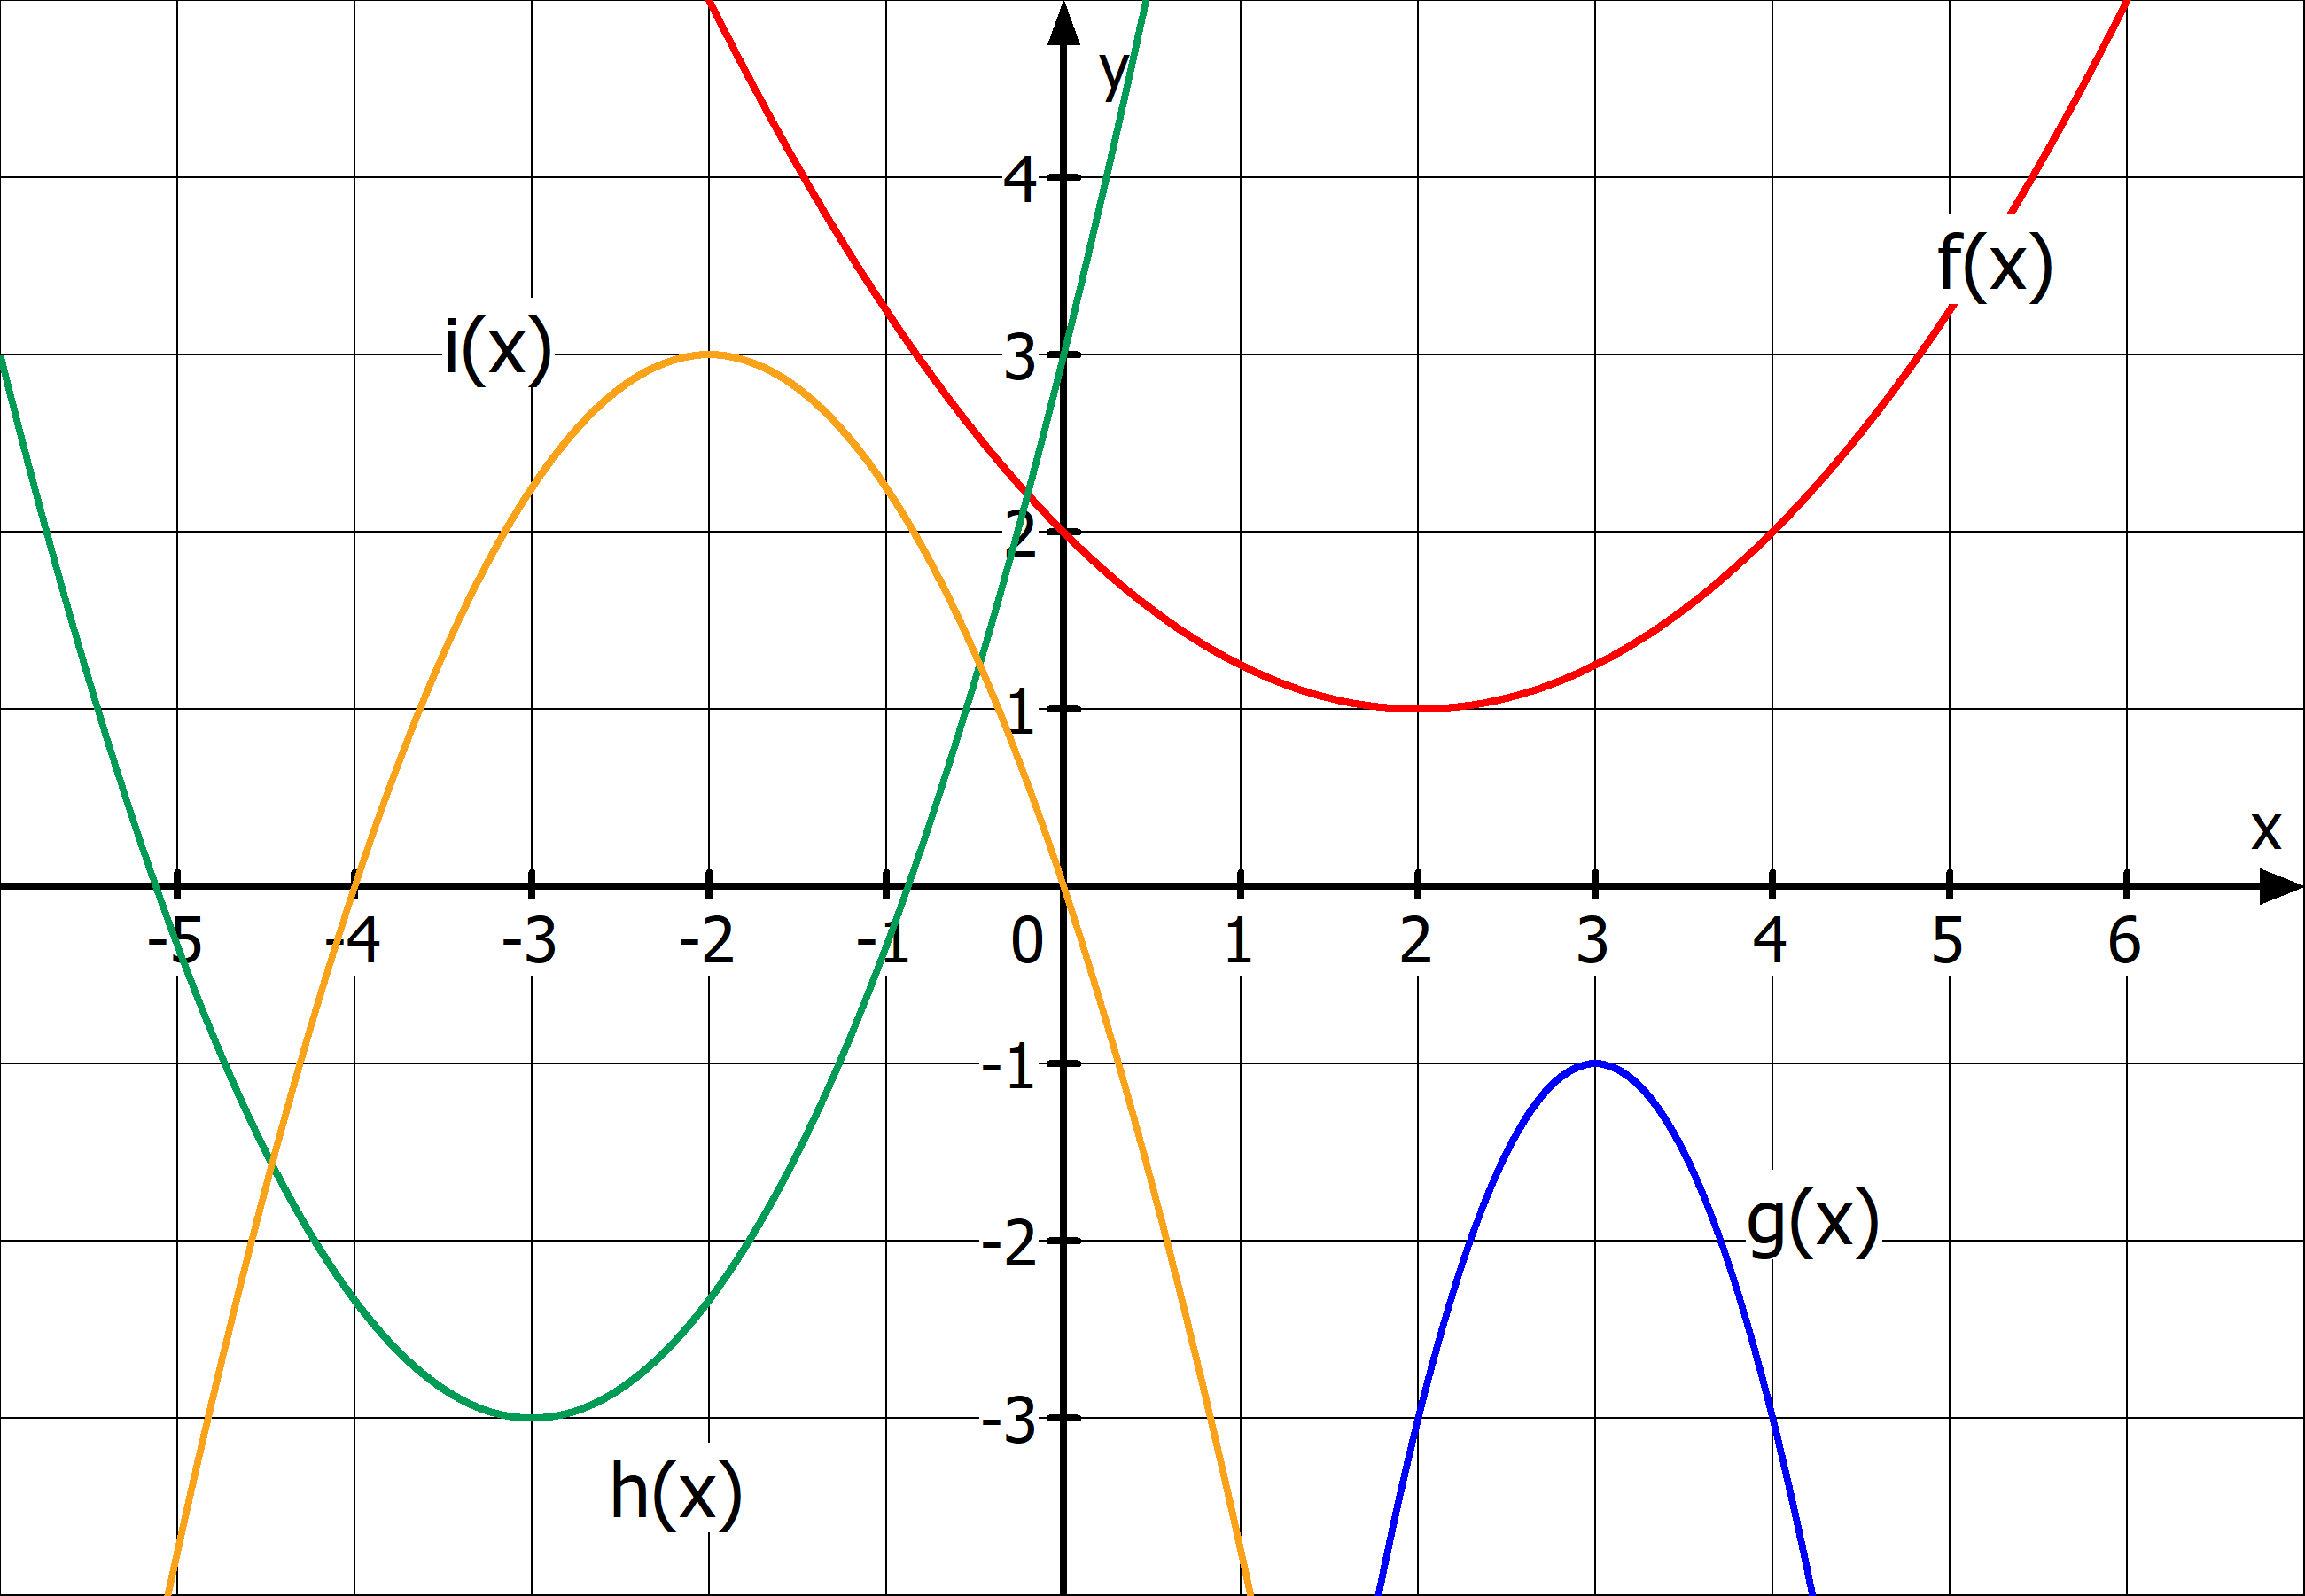
\includegraphics[width=\linewidth]{\quadFkt/pics/scheitelA1.png}
	\end{minipage}%
\end{Exercise}

\begin{Exercise}[title={Stelle jeweils die Funktionsgleichung auf und skizziere das Schaubild}, label=scheitelformA2]
	\begin{enumerate}[label=\alph*)]
		\item Die Normalparabel wird mit dem Faktor 4 gestreckt um 2 Einheiten nach links und um 4 Einheiten nach unten verschoben.
		\item Die Normalparabel wird mit dem Faktor 0,5 gestreckt, an der x-Achse gespiegelt, um 1 Einheiten nach rechts und um 2 Einheiten nach unten verschoben.
		\item Die Normalparabel wird mit dem Faktor 2 gestreckt, um 2,5 Einheiten nach links, um 3,5 Einheiten nach oben verschoben und zuletzt an der x-Achse gespiegelt.
	\end{enumerate}
\end{Exercise}
\begin{Exercise}[title={Beschreibe wie man die jeweilige Parabel aus der Normalparabel erhält.}, label=scheitelformA3]
	\begin{enumerate}[label=\alph*)]
		\item \(f(x)=5(x-1)^2+2\) \quad b) \(g(x)=-(x+3)^2-2,5\) \quad c) \(h(x)=-\tfrac{2}{3}\left(x-\tfrac{3}{4}\right)^2+\tfrac{5}{7}\)
	\end{enumerate}
\end{Exercise}
\begin{Exercise}[title={Stelle die Funktionsgleichung auf}, label=scheitelformA4]
	\begin{enumerate}[label=\alph*)]
		\item Das Schaubild von \(f(x)=3(x-4)^2+2\) wird um 5 Einheiten nach links und 2 Einheiten nach oben verschoben und dann an der x-Achse gespiegelt.
		\item Das Schaubild von \(g(x)=-(x+2)^2-3\) wird um 5 Einheiten nach rechts und 2 Einheiten nach unten verschoben und dann an der y-Achse gespiegelt.
	\end{enumerate}
\end{Exercise}\newpage

\begin{Answer}[ref=scheitelformA1]

	\begin{enumerate}[label=\alph*)]
		\item \textcolor{red}{\(f(x)=\tfrac{1}{4}\left(x-2\right)^2+1\)} \quad b) \textcolor{blue}{\(g(x)=-2\left(x-3\right)^2-1\)} \setcounter{enumi}{2}
		\item \textcolor{ForestGreen}{\(h(x)=\tfrac{2}{3}\left(x+3\right)^2-3\)} \quad d) \textcolor{YellowOrange}{\(i(x)=-\tfrac{3}{4}\left(x+2\right)^2+3\)}
	\end{enumerate}
	Hinweis: Bestimme \(x_S\) und \(y_S\) aus der Position des Scheitels. Den Streckfaktor \(a\) kann man dann mittels einer Punktprobe bestimmen (nicht den Scheitel als Punkt verwenden).
\end{Answer}

\begin{Answer}[ref=scheitelformA2]

	\begin{minipage}{\linewidth}\centering
		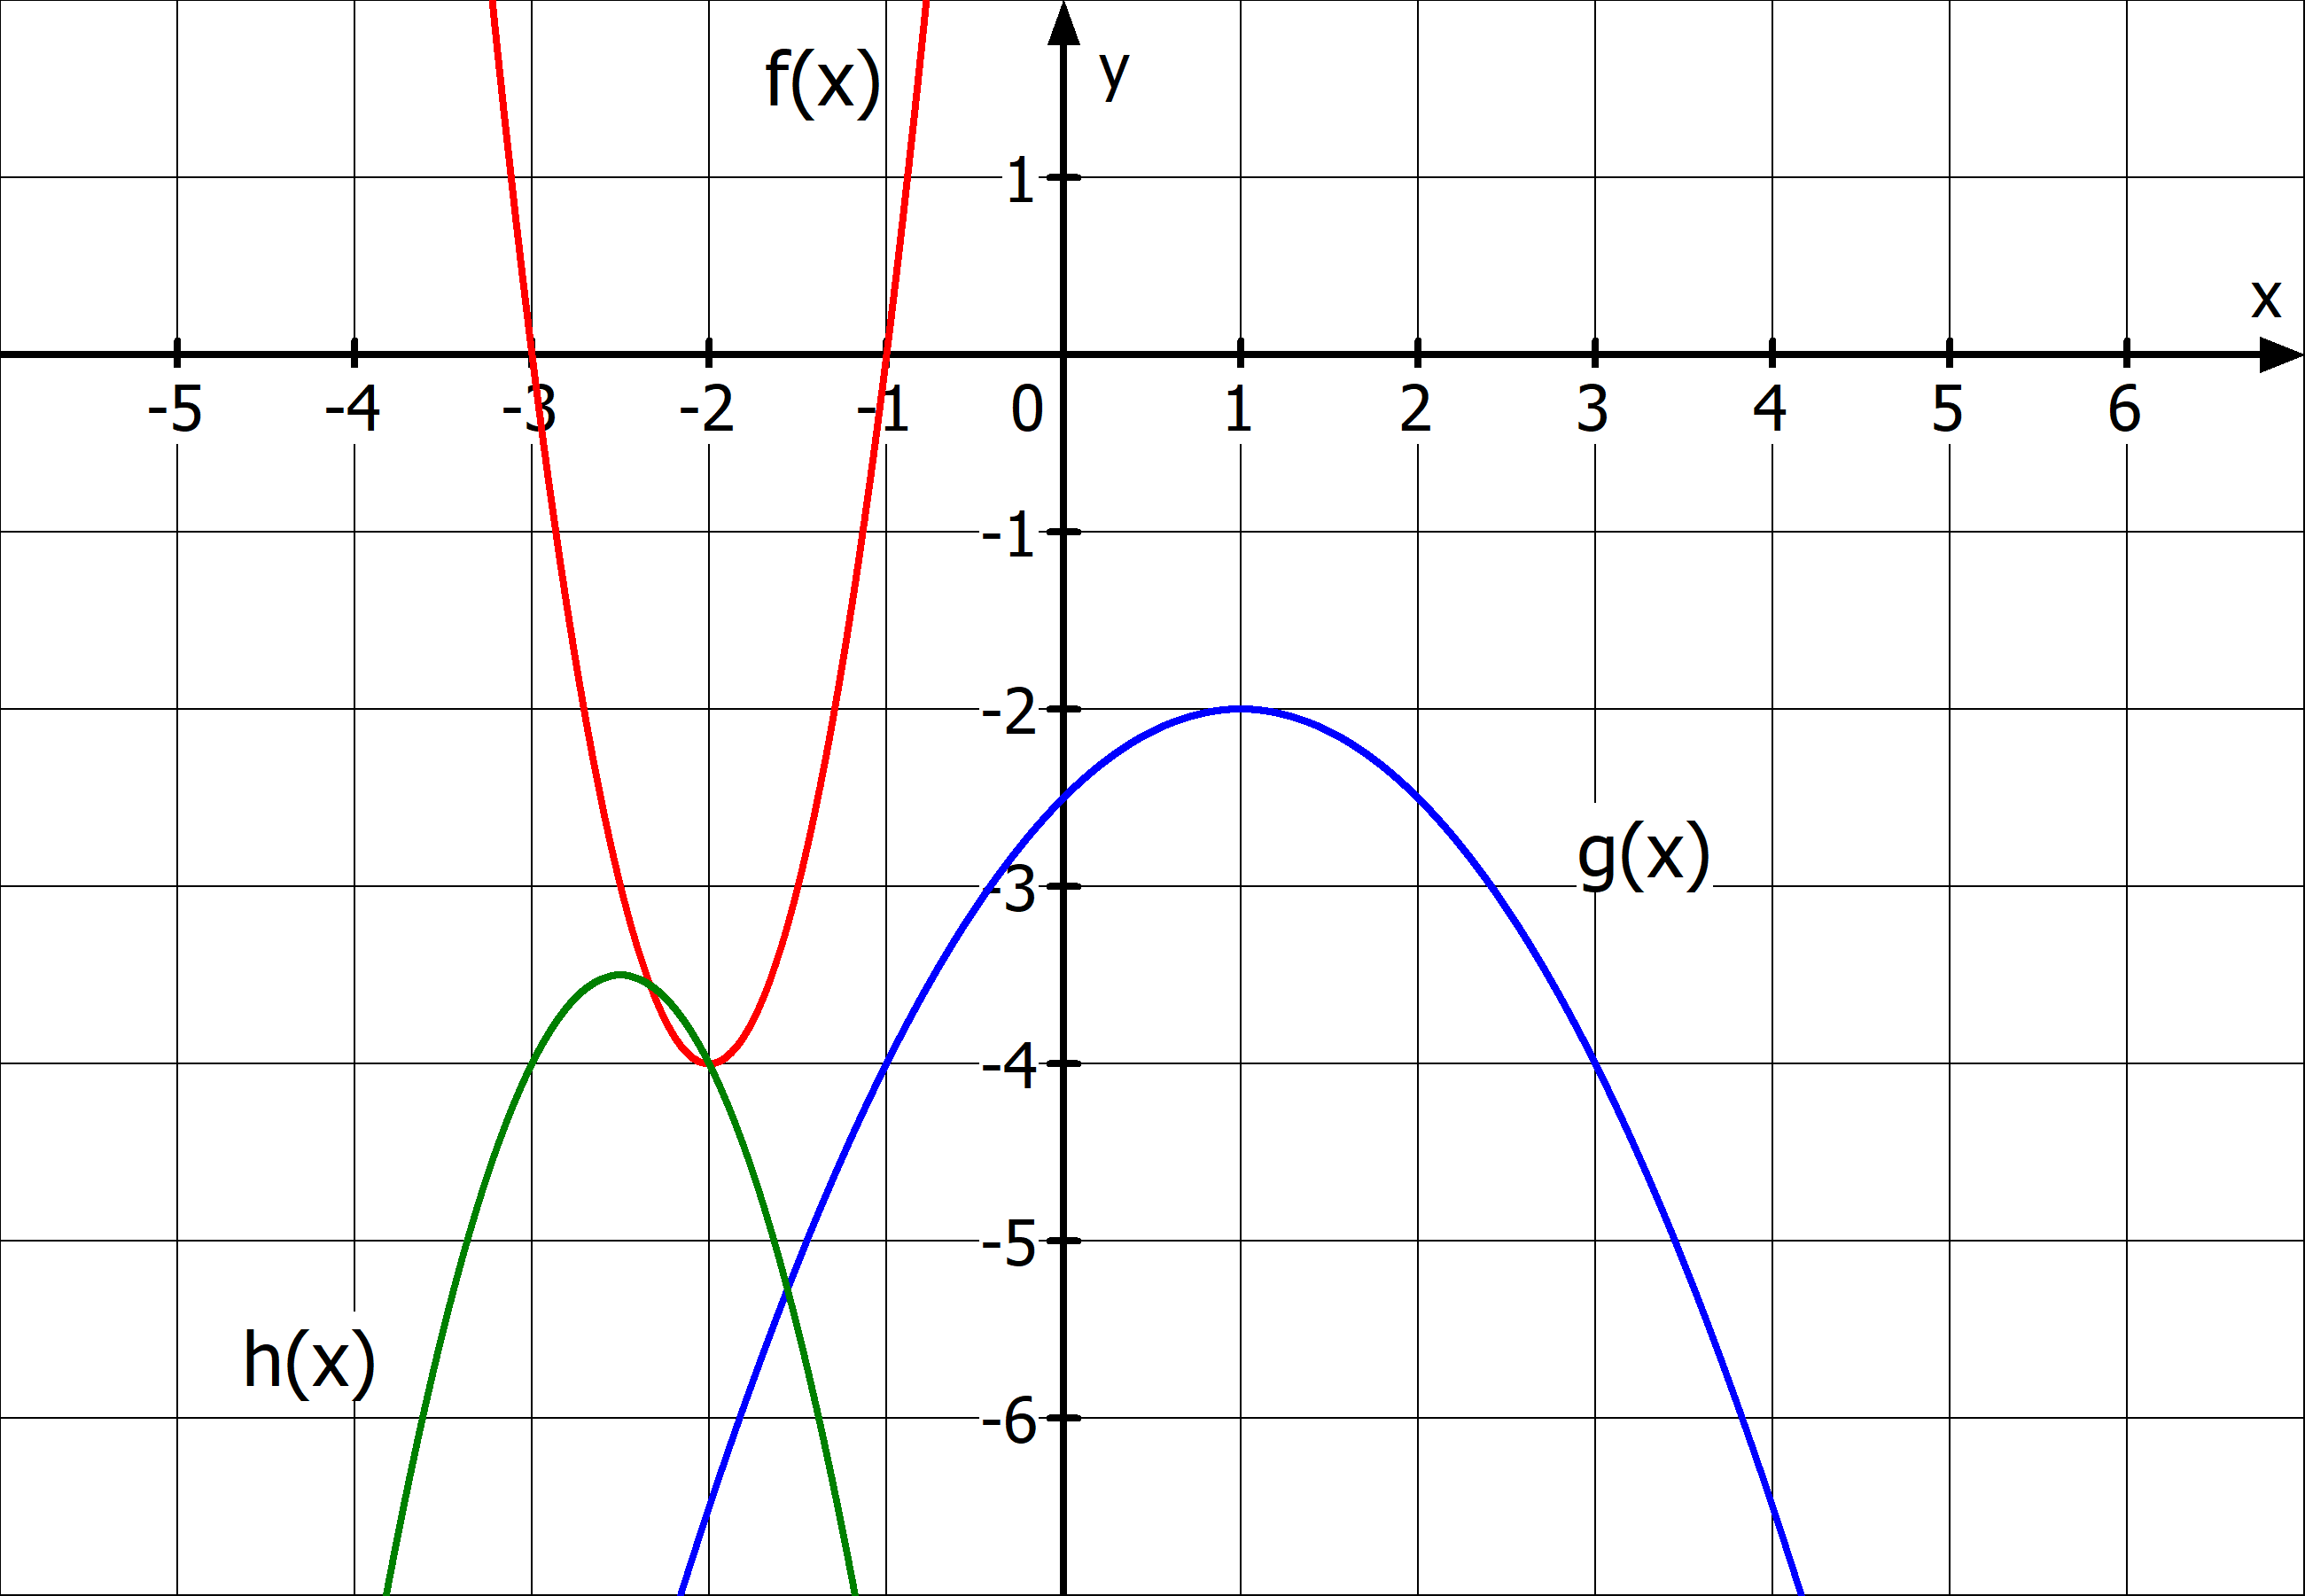
\includegraphics[width=\linewidth]{\quadFkt/pics/scheitelA2.png}
	\end{minipage}\vspace{.1cm}
	\begin{enumerate}[label=\alph*)]
		\item \textcolor{red}{\(f(x)=4\left(x+2\right)^2-4\)}
		\quad b) \textcolor{blue}{\(g(x)=-\tfrac{1}{2}\left(x-1\right)^2-2\)} \quad c) \textcolor{ForestGreen}{\(h(x)=-2\left(x+2,5\right)^2-3,5\)}
	\end{enumerate}
\end{Answer}
\begin{Answer}[ref=scheitelformA3]

	\begin{enumerate}[label=\alph*)]
		\item Die Normalparabel wird mit dem Faktor 5 gestreckt, um 1 Einheit nach rechts und 2 Einheiten nach oben verschoben.
		\item Die Normalparabel wird an der x-Achse gespiegelt, um 3 Einheiten nach links und 2,5 Einheiten nach unten verschoben.
		\item Die Normalparabel wird mit dem Faktor 1,5 gestreckt, an der x-Achse gespiegelt, um 0,75 Einheiten nach rechts und \(\tfrac{5}{7}\) Einheiten nach oben verschoben.
	\end{enumerate}
\end{Answer}
\begin{Answer}[ref=scheitelformA4]

	\begin{enumerate}[label=\alph*)]
		\item \(f_v(x)=-3\left(x+1\right)^2-4\) \quad b) \(g_v(x)=-\left(x+3\right)^2-5\)
	\end{enumerate}
\end{Answer}\newpage